\documentclass[a4paper,12pt, master]{etf}

\usepackage[intlimits]{amsmath}
\usepackage{amsmath, amsfonts, amssymb, graphicx, systeme}

\usepackage[english]{babel}
\usepackage[T1]{fontenc}
\usepackage[utf8]{inputenc}
\usepackage{algorithm}
  \makeatletter
  \renewcommand{\ALG@name}{Algorithm}
  \makeatother
\usepackage{algpseudocode}
\usepackage{float}
\usepackage[hidelinks]{hyperref}
\usepackage{subcaption}
\usepackage{longtable}

% list of abbreviations, styled like the lists of figures and tables of the class
\makeatletter
\newcommand\listabbrevname{List of Abbreviations}
\newcommand\listofabbreviations{%
    \chapter*{\listabbrevname}%
    \@mkboth{\MakeUppercase\listabbrevname}{\MakeUppercase\listabbrevname}%
    \begin{longtable}{@{}p{0.2\textwidth}p{0.75\textwidth}@{}}
    \input{abbreviations}
    \end{longtable}}
\makeatother



\addto\captionsserbian{%
\renewcommand{\bibname}%
{Literature}%
}


\title{Efficient Hardware Implementation of a Mixed-Radix Fast Fourier Transform Algorithm}
\author{Lazar Dobrić}
\indeks{2024/3087}
\date{september 2026.}
\mentor{dr Vladimir Petrović, assistant professor}
\predmet{Digital Signal Processors}

\begin{document}

\maketitle

\begin{abstract}
In this work, the theoretical background of the mixed-radix Fast Fourier Transform (FFT) algorithm is presented. The necessary algorithms for its implementation are analyzed. A Single-path Delay Feedback (SDF) hardware architecture for the FFT is simulated in software. The hardware implementation of the FFT is realized on a Field-Programmable Gate Array (FPGA) chip.
\end{abstract}

\begin{keywords}
Mixed-radix FFT, SDF architecture, FPGA
\end{keywords}

\tableofcontents

\chapter{Introduction}

Modern communication systems like 4G LTE, 5G or WiFi face a number of problems that are caused by the nature of wireless communication. One cure for the majority of them is the Orthogonal Frequency Division Multiplexing (OFDM) modulation scheme. The core of OFDM is the Discrete Fourier Transform (DFT), and the tool used to efficiently calculate it is the Fast Fourier Transform (FFT). High data rates imply hardware acceleration and high parallelization of the FFT. In addition, the OFDM modulation scheme found in 4G Long Term Evolution (LTE) and 5G New Radio (NR) requires the mixed-radix FFT to be calculated efficiently.

Hardware acceleration of such algorithms is usually realized as Application-Specific Integrated Circuit (ASIC) implementations, meaning a fixed chip design for a specific algorithm satisfying the standard requirements.
These systems go through a number of problems and iterations in each of their generations, so the standards evolve and new requirements are added. The constant evolution of standards and requirements forces the hardware acceleration of algorithms to change with them. Making a new ASIC for each new standard would be too expensive and time-consuming, so a software implementation or hardware acceleration on Field-Programmable Gate Arrays (FPGAs) is a more suitable solution. A software implementation requires significant overhead that introduces latency, so FPGA acceleration is the preferred solution.

To implement the mixed-radix FFT on an FPGA, a hardware architecture that is efficient and flexible enough is needed. Many details need consideration, such as efficient utilization of DSP resources, as well as choosing the right type of memory as per the requirements of the algorithm.

The aim of this work is to present an implementation of the mixed-radix FFT architecture that is efficient and flexible enough to be used in a communication system. Based on the 5G NR standard requirements, the architecture is designed, modeled and implemented on an FPGA, but with flexibility in mind, enabling arbitrary transform sizes to be supported. Finally, the performance and the mapping of the architecture to the available resources are presented.

The modeling of the architecture is done using the Python programming language and represents the bit-exact software fixed-point model of the implementation. The implementation is done in VHDL using GHDL for simulation and the Vivado 2022.2 design suite for synthesis and place and route.

In chapter \ref{ch:theoretical_background}, the theoretical background necessary for understanding the architecture and implementation of the mixed-radix FFT algorithm is discussed. OFDM is introduced and the 5G NR standard physical layer is described, from which the set of required transform sizes is derived. Then the theory behind the FFT is presented, from the radix-2 algorithm to the mixed-radix decomposition, the digit inversion of the output order and the inverse transform. After that, fixed-point arithmetic is introduced.

Chapter \ref{ch:hardware_architecture} describes the hardware architecture. It starts from the streaming single-path delay feedback architecture and extends it to a chain of reconfigurable stages that covers all required sizes with one datapath, and then breaks a stage down into its units -- the preadders, the twiddle factor unit, the rotator, the FIFOs and the control -- together with the flow control between the stages and the top-level control with its register interface.

Chapter \ref{ch:software_model} describes the software reference model written in Python. The fixed-point formats of the datapath, the coefficients and the twiddle factors are selected here with the target FPGA resources in mind, and the quantization noise of the resulting design is evaluated over all supported sizes.

Chapter \ref{ch:results} presents the results of the implementation. The verification flow and the block design used on the target board are described, the memory budget that decides the order of the stages is worked out, and the resource utilization, the timing and the measurements on the board are reported.

Chapter \ref{chap:future_work} discusses two improvements of the design that were identified but not implemented: the reduction of the twiddle factor storage and a hardware unit for the reordering of the output samples into natural order. Finally, chapter \ref{ch:conclusion} summarizes the work.


\chapter{Theoretical background}
\label{ch:theoretical_background}

In this chapter, the theoretical background necessary for understanding the architecture and implementation of the mixed-radix FFT algorithm will be discussed.

\section{OFDM}

Modern communication systems face a number of problems, the most significant being:
- high data rates,
- limited spectral bandwidth,
- urban environments,
- users moving through space.

To meet the requirements of modern life, they have to provide extremely high data rates through wireless communication in demanding urban environments full of radio-reflective materials and densely packed buildings. Modern users expect to be able to use their phones while walking down a street or riding a bus.

All these requirements manifest themselves as issues when designing such a system. High data rates within a limited spectral bandwidth require high spectral efficiency. Wave propagation in concrete environments and moving users introduce multipath propagation, frequency-selective fading and the Doppler effect.

The issue arises when a modulation scheme that modulates symbols at a symbol rate $1/T$ matching the bandwidth $W$ is used in a band where frequency-selective fading is present. Different frequency components of a received symbol then suffer different fading as the signal passes through the channel. To suppress this, one could use Frequency Division Multiplexing (FDM), where the whole bandwidth $W$ is split into $N$ subchannels used in parallel. If each such subchannel is narrow enough, the channel frequency response is essentially constant across it, which solves the fading issue. But splitting a single channel into multiple narrower subchannels requires additional guard bands between them to ensure that there is no overlap, so that inter-carrier interference is kept low enough. Because of the guard bands, the spectral efficiency drops compared to the original single-channel configuration.


5G and modern WiFi systems aim to solve these issues by using OFDM. A single band of width $W$ is split into $N$ subchannels of width $W/N$. By selecting the symbol rate $1/T$ in each of the subchannels to be equal to the frequency separation $\Delta f$ of the adjacent subcarriers, the subcarriers become orthogonal over the symbol interval $T$. Now, if $N$ is chosen such that $\Delta f = W/N$ is small enough, the channel frequency response $C(f)$ is essentially constant across each of the subchannels. This way it is possible to reach transmission rates close to the channel capacity and minimize the effect of frequency-selective fading.

Recall that the DFT essentially calculates the coefficients of a linear combination of complex exponentials that are orthogonal over an interval of $N$ samples. The orthogonality of the subcarriers therefore allows efficient modulation and demodulation using the DFT, calculated with the FFT algorithm.

\subsection{5G NR standard physical layer}

The physical layer of the 5G NR standard is defined by 3GPP in \cite{17}. It specifies cyclic-prefix OFDM (CP-OFDM) as the waveform in both downlink and uplink, with QPSK, 16-QAM, 64-QAM and 256-QAM used to modulate the individual subcarriers. Among all the physical layer parameters, the most important ones for the OFDM modulator and demodulator are the subcarrier spacing $\Delta f$ and the number of used subcarriers, since these two directly determine the required DFT size and the sampling rate of the system.

Unlike 4G LTE, which uses a single fixed subcarrier spacing of $15\,\mathrm{kHz}$, 5G NR defines a scalable numerology. The numerology is selected by the parameter $\mu$ and the subcarrier spacing is given by
\begin{equation}
    \Delta f = 2^{\mu} \cdot 15\,\mathrm{kHz}, \quad \mu \in \{0, 1, 2, 3, 4\}.
\label{eq:nr_numerology}
\end{equation}
The corresponding OFDM symbol duration is $T = 1/\Delta f$. Narrow subcarrier spacings ($15$ and $30\,\mathrm{kHz}$) are used in the FR1 frequency range (sub-6 GHz bands) where large cells and long channel delay spreads require a long cyclic prefix, while wide spacings ($120\,\mathrm{kHz}$ and above) are used in the FR2 range (millimeter-wave bands) where robustness to phase noise and Doppler shift is needed. The supported numerologies are summarized in Table \ref{tab:nr_numerologies}.

\begin{table}[htb]
\centering
\caption{5G NR numerologies \cite{17}.}
\medskip
\label{tab:nr_numerologies}
\begin{tabular}{c | c | c | c}
\hline
$\mu$ & $\Delta f$ [kHz] & Symbol duration $T$ [$\mu$s] & Frequency range\\
\hline
\hline
0 & 15 & 66.67 & FR1\\
\hline
1 & 30 & 33.33 & FR1\\
\hline
2 & 60 & 16.67 & FR1, FR2\\
\hline
3 & 120 & 8.33 & FR2\\
\hline
4 & 240 & 4.17 & FR2 (synchronization only)\\
\hline
\end{tabular}
\end{table}

In the frequency domain, subcarriers are grouped into resource blocks (RB), where one RB consists of 12 consecutive subcarriers. A carrier may contain at most 275 RBs, i.e. 3300 active subcarriers. The number of RBs for each combination of channel bandwidth and subcarrier spacing is specified in \cite{18}. For example, a $100\,\mathrm{MHz}$ carrier with $\Delta f = 30\,\mathrm{kHz}$ contains 273 RBs, which amounts to 3276 active subcarriers.

\subsection{FFT sizes and radices required by 5G NR}
\label{subsec:nr_fft_sizes}

OFDM modulation and demodulation are implemented as an IDFT and a DFT, calculated using the FFT algorithm. The transform size $N$ must be larger than or equal to the number of active subcarriers (if larger, the remaining inputs are set to zero and act as guard bands). The choice of $N$ also determines the sampling rate of the baseband signal,
\begin{equation}
    f_s = N \cdot \Delta f.
\label{eq:nr_sampling_rate}
\end{equation}
The standard itself is defined around a reference transform size of $N = 4096$: the basic time unit of NR is $T_c = 1/(\Delta f_{max} \cdot N_f)$, where $\Delta f_{max} = 480\,\mathrm{kHz}$ and $N_f = 4096$ \cite{17}. Transform sizes for other configurations are an implementation choice and are typically chosen as the smallest size that fits all active subcarriers. Table \ref{tab:nr_fft_sizes} lists transform sizes and sampling rates for several typical NR carrier configurations.

\begin{table}[htb]
\centering
\caption{Typical FFT sizes for 5G NR carrier configurations \cite{18}.}
\medskip
\label{tab:nr_fft_sizes}
\begin{tabular}{c | c | c | c | c}
\hline
Bandwidth [MHz] & $\Delta f$ [kHz] & Active subcarriers & $N$ & $f_s$ [MHz]\\
\hline
\hline
5 & 15 & 300 & 512 & 7.68\\
\hline
10 & 15 & 624 & 1024 & 15.36\\
\hline
15 & 15 & 948 & 1536 & 23.04\\
\hline
20 & 15 & 1272 & 2048 & 30.72\\
\hline
50 & 30 & 1584 & 2048 & 61.44\\
\hline
80 & 30 & 2604 & 3072 & 92.16\\
\hline
100 & 30 & 3276 & 4096 & 122.88\\
\hline
400 & 120 & 3168 & 4096 & 491.52\\
\hline
\end{tabular}
\end{table}

Most of the required transform sizes are powers of two ($512$, $1024$, $2048$, $4096$), which can be calculated using only radix-2 stages (or, equivalently, radix-4 and radix-8 stages). However, for some configurations the number of active subcarriers falls just above a power of two, and using the next power of two would be wasteful. For a $15\,\mathrm{MHz}$ carrier with $\Delta f = 15\,\mathrm{kHz}$ there are 948 active subcarriers, so $N = 1024$ is too small, while $N = 2048$ would double the sampling rate to $30.72\,\mathrm{MHz}$. Instead, the size $N = 1536 = 3 \cdot 2^9$ is used, which reduces the sampling rate by $25\%$ compared to $N = 2048$. Similarly, $N = 3072 = 3 \cdot 2^{10}$ is used for an $80\,\mathrm{MHz}$ carrier with $\Delta f = 30\,\mathrm{kHz}$ instead of $N = 4096$. A lower sampling rate directly relaxes the throughput requirements of the FFT hardware and of the digital front-end that follows it. Supporting these sizes requires one radix-3 stage in addition to the radix-2 stages.

An even stronger requirement for mixed-radix processing comes from the NR uplink. Besides CP-OFDM, the uplink optionally uses DFT-spread OFDM (DFT-s-OFDM), also called transform precoding, where the modulation symbols are first passed through a DFT before being mapped onto the subcarriers of the OFDM modulator. This spreading lowers the Peak-to-Average Power Ratio (PAPR) of the transmitted signal, which improves the power amplifier efficiency of coverage-limited user devices. The size of the spreading DFT equals the number of allocated subcarriers,
\begin{equation}
    M = 12 \cdot M_{RB},
\label{eq:nr_dft_size}
\end{equation}
where $M_{RB}$ is the number of allocated resource blocks. To guarantee that this DFT can always be calculated efficiently, the standard \cite{17} restricts the allocation to values of the form
\begin{equation}
    M_{RB} = 2^{\alpha_2} \cdot 3^{\alpha_3} \cdot 5^{\alpha_5},
\label{eq:nr_rb_constraint}
\end{equation}
where $\alpha_2$, $\alpha_3$ and $\alpha_5$ are non-negative integers. There are exactly 53 such values of $M_{RB}$ not exceeding the maximum of 275 RBs, listed in Table \ref{tab:nr_dft_sizes}. The corresponding DFT sizes range from $M = 12$ (1 RB) to $M = 3240$ (270 RBs), and every one of them factorizes exclusively into the factors 2, 3 and 5.

\begin{table}[htb]
\centering
\caption{The 53 allowed values of $M_{RB}$ for DFT-s-OFDM in 5G NR \cite{17}.}
\medskip
\label{tab:nr_dft_sizes}
\begin{tabular}{c c c c c c c c c c}
\hline
1 & 2 & 3 & 4 & 5 & 6 & 8 & 9 & 10 & 12\\
15 & 16 & 18 & 20 & 24 & 25 & 27 & 30 & 32 & 36\\
40 & 45 & 48 & 50 & 54 & 60 & 64 & 72 & 75 & 80\\
81 & 90 & 96 & 100 & 108 & 120 & 125 & 128 & 135 & 144\\
150 & 160 & 162 & 180 & 192 & 200 & 216 & 225 & 240 & 243\\
250 & 256 & 270 & & & & & & & \\
\hline
\end{tabular}
\end{table}

Therefore, an FFT processor intended for a 5G NR modem must support all transform sizes of the form
\begin{equation}
    N = 2^{a} \cdot 3^{b} \cdot 5^{c},
\label{eq:nr_fft_sizes_form}
\end{equation}
covering both the OFDM modulator sizes $\{512, 1024, 1536, 2048, 3072, 4096\}$ and the 53 transform precoding sizes $M = 12 \cdot M_{RB}$. This is exactly the motivation for the mixed-radix FFT architecture presented in this work: a single hardware architecture combining radix-2, radix-3 and radix-5 butterfly stages can cover all transform sizes required by the 5G NR physical layer.

All 53 transform sizes of the DFT performed before the OFDM modulator are listed in Table \ref{tab:nr_precoding_sizes}.

\begin{table}[htb]
\centering
\caption{The 53 transform precoding sizes $M = 12 \cdot M_{RB}$ for DFT-s-OFDM in 5G NR \cite{17}.}
\medskip
\label{tab:nr_precoding_sizes}
\begin{tabular}{c c c c c c c c c c}
\hline
12 & 24 & 36 & 48 & 60 & 72 & 96 & 108 & 120 & 144\\
180 & 192 & 216 & 240 & 288 & 300 & 324 & 360 & 384 & 432\\
480 & 540 & 576 & 600 & 648 & 720 & 768 & 864 & 900 & 960\\
972 & 1080 & 1152 & 1200 & 1296 & 1440 & 1500 & 1536 & 1620 & 1728\\
1800 & 1920 & 1944 & 2160 & 2304 & 2400 & 2592 & 2700 & 2880 & 2916\\
3000 & 3072 & 3240 & & & & & & & \\
\hline
\end{tabular}
\end{table}

\section{FFT}

\subsection{FT}

The Fourier Transform $F(\omega)$ is a mathematical transformation, expressed as (\ref{ft_formula}), that transforms a continuous complex signal $f(t)$ from the time to the frequency domain. It is a tool for the analysis of the frequency content of a signal.

\begin{equation}
    F(\omega) = \int_{-\infty}^{\infty} f(t) e^{-j \omega t} dt
\label{ft_formula}
\end{equation}

Digital systems process discrete signals, so a more useful tool for them is the DFT, expressed as (\ref{dft_formula}), which transforms a discrete complex signal $x[n]$ ($n \in \{0, 1, \ldots, N-1\}$) from the time to the frequency domain, where $X[k]$ ($k \in \{0, 1, \ldots, N-1\}$) are the coefficients that multiply the basis complex exponentials of the DFT, and $N$ is the number of samples in the signal.

\begin{equation}
    X[k] = \sum_{n=0}^{N-1} x[n] e^{-j \frac{2\pi}{N} n k}
\label{dft_formula}
\end{equation}

The complex factors $e^{-j \frac{2\pi}{N} n k}$ are usually called twiddle factors. They are commonly denoted as $W_N^{nk}$, so that:

\begin{equation}
    W_N^{nk} = e^{-j \frac{2\pi}{N} n k}.
\label{twiddle_factor_formula}
\end{equation}

The DFT can then be expressed as:

\begin{equation}
    X[k] = \sum_{n=0}^{N-1} x[n] W_N^{nk}.
\label{dft_formula_2}
\end{equation}

Calculation of the DFT by its definition has $O(N^2)$ complexity. This is because for each $k$ from $0$ to $N-1$ there are $N$ complex multiplications and $N-1$ complex additions. This can be reduced to $O(N \log N)$ complexity by using FFT algorithms.

\subsection{FFT}
To reduce the complexity of the DFT calculation, FFT algorithms are used. Many different FFT algorithms exist, but the most common one is the Cooley-Tukey algorithm.

The Cooley-Tukey algorithm is based on the fact that the calculations of some terms in the DFT can be reused for the calculations of other terms by rearranging the terms. This way, the number of calculations is reduced.
The rearrangement can be done on the input samples or on the output samples; this is called decimation in time (DIT) or decimation in frequency (DIF), respectively. In the following, we explain the algorithm that uses DIF for the rearrangement.

A DFT of length $N$ can be factorized into $N = N_1 N_2$, where $N_1$ and $N_2$ are natural numbers. Thus, a DFT of length $N$ can be calculated as $N_1$ DFTs of length $N_2$. If $N_1 = N_2$, the DFT of length $N$ can be calculated as two DFTs of length $N/2$. This is a special case known as the radix-2 FFT.

The above can be expressed mathematically as:
\begin{equation}
\begin{split}
    X[k] &= \sum_{n=0}^{N-1} x[n] \cdot W_N^{nk} \\
    &= \sum_{n=0}^{N_1-1} x[n] \cdot W_N^{nk} + \sum_{n=N_1}^{N-1} x[n] \cdot W_N^{nk} \\
    &= \sum_{n=0}^{N/2-1} x[n] \cdot W_N^{nk} + \sum_{n=N/2}^{N-1} x[n] \cdot W_N^{nk} \\
    &= \sum_{n=0}^{N/2-1} x[n] \cdot W_N^{nk} + \sum_{n=0}^{N/2-1} x[n + N/2] \cdot W_N^{(n + N/2)k} \\
    &= \sum_{n=0}^{N/2-1} x[n] \cdot W_N^{nk} + W_N^{N/2k}\cdot\sum_{n=0}^{N/2-1} x[n + N/2] \cdot W_N^{nk}.
\label{dft_radix2_0}
\end{split}
\end{equation}

Twiddle factors satisfy the identity described in (\ref{twiddle_factor_identity}).

\begin{equation}
    W_N^{2nk} = e^{-j \frac{2\pi}{N} 2nk} = e^{-j \frac{2\pi}{N/2} nk} = W_{N/2}^{nk}.
\label{twiddle_factor_identity}
\end{equation}

Thus, by using the identity (\ref{twiddle_factor_identity}) and substituting $k=2m$ ($m \in \{0, 1, \ldots, N/2-1\}$), we calculate the even-indexed output samples $X[2m]$ as:

\begin{equation}
\begin{split}
    X[2m] &= \sum_{n=0}^{N/2-1} x[n] \cdot W_N^{n\cdot2m} + W_N^{N/2 \cdot 2m}\cdot\sum_{n=0}^{N/2-1} x[n + N/2] \cdot W_N^{n \cdot 2m} \\
    &= \sum_{n=0}^{N/2-1} x[n] \cdot W_{N/2}^{nm} + W_N^{Nm}\cdot\sum_{n=0}^{N/2-1} x[n + N/2] \cdot W_{N/2}^{nm} \\
    &= \sum_{n=0}^{N/2-1} (x[n] \cdot W_{N/2}^{nm} + W_N^{Nm}\cdot x[n + N/2] \cdot W_{N/2}^{nm}) \\
    &= \sum_{n=0}^{N/2-1} (x[n] + x[n + N/2]) \cdot W_{N/2}^{nm}, \ W_N^{Nm} = 1.
\label{dft_radix2_1}
\end{split}
\end{equation}

If we denote $G(m) = X[2m]$, then $G(m)$ can be viewed as a DFT of the sequence $g(n) = x[n] + x[n + N/2]$ of length $N/2$.

Similarly, substituting $k=2m+1$ gives the odd-indexed output samples $X[2m+1]$:
\begin{equation}
\begin{split}
    X[2m+1] &= \sum_{n=0}^{N/2-1} x[n] \cdot W_N^{n\cdot(2m+1)} \\
    &\quad + W_N^{N/2 \cdot (2m+1)}\cdot\sum_{n=0}^{N/2-1} x[n + N/2] \cdot W_N^{n \cdot (2m+1)} \\
    &= \sum_{n=0}^{N/2-1} x[n] \cdot W_{N}^{n\cdot2m} \cdot W_{N}^{n} \\
    &\quad + W_N^{Nm}\cdot W_N^{N/2} \cdot\sum_{n=0}^{N/2-1} x[n + N/2] \cdot W_{N}^{n\cdot 2m} \cdot W_N^{n} \\
    &= \sum_{n=0}^{N/2-1} x[n] \cdot W_{N/2}^{n\cdot m} \cdot W_{N}^{n} \\
    &\quad + W_N^{Nm}\cdot W_N^{N/2} \cdot\sum_{n=0}^{N/2-1} x[n + N/2] \cdot W_{N/2}^{n\cdot m} \cdot W_N^{n} \\
    &= \sum_{n=0}^{N/2-1} ((x[n] - x[n + N/2]) \cdot W_{N}^{n}) \cdot W_{N/2}^{n\cdot m}, \ W_{N}^{N/2} = -1. \\
\label{dft_radix2_2}
\end{split}
\end{equation}

If we denote $H(m) = X[2m+1]$, then $H(m)$ can be viewed as a DFT of the sequence $h(n) = (x[n] - x[n + N/2]) \cdot W_N^{n}$ of length $N/2$.

Equations (\ref{dft_radix2_1}) and (\ref{dft_radix2_2}) are represented graphically in Figure \ref{fig:radix2_fft_0_diag} for $N=8$.

\begin{figure}[htbp]
    \centering
    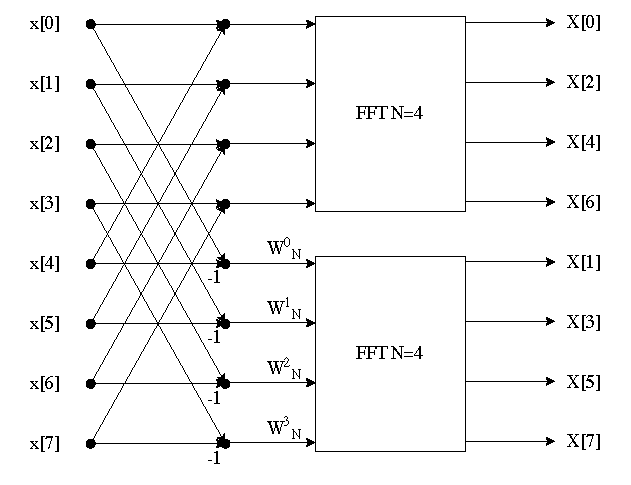
\includegraphics[width=0.8\textwidth]{figs/radix2_fft_0.pdf}
    \caption{Graphical representation of the equations (\ref{dft_radix2_1}) and (\ref{dft_radix2_2}) for $N=8$.}
    \label{fig:radix2_fft_0_diag}
\end{figure}

If the length of the DFT is a power of two, the algorithm can be applied recursively until the base case of length 2 is reached.

Then, the diagram in Figure \ref{fig:radix2_fft_0_diag} can be presented as in Figure \ref{fig:radix2_fft_1_diag}.

\begin{figure}[htbp]
    \centering
    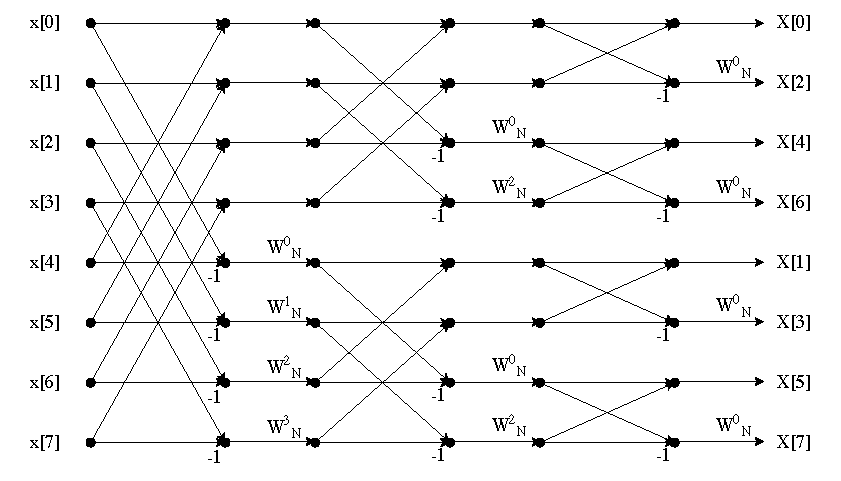
\includegraphics[width=1.0\textwidth]{figs/radix2_fft_1.pdf}
    \caption{Graphical representation of the equations (\ref{dft_radix2_1}) and (\ref{dft_radix2_2}) for $N=8$.}
    \label{fig:radix2_fft_1_diag}
\end{figure}

The basic element of this diagram is called a butterfly. It is the basic building block of the FFT algorithm and essentially calculates the DFT of two samples. It is represented in Figure \ref{fig:radix2_fft_2_diag}.

\begin{figure}[htbp]
    \centering
    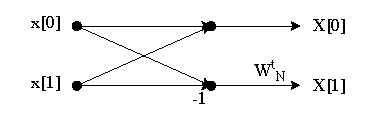
\includegraphics[width=0.6\textwidth]{figs/radix2_fft_2.pdf}
    \caption{Graphical representation of the radix-2 butterfly.}
    \label{fig:radix2_fft_2_diag}
\end{figure}

A line with the symbol $W_N^{t}$ above it represents a complex multiplication, and a node with two inputs and an output represents a complex addition.
By observing the diagram in Figure \ref{fig:radix2_fft_2_diag}, it can be seen that each stage of the FFT requires $N$ complex additions to combine the even and odd samples and $N/2$ complex multiplications to multiply half of the samples by the twiddle factors. The radix-2 FFT requires $\log_2 N$ stages, so the complexity of the FFT algorithm is $O(N \log N)$.

The final radix-2 FFT algorithm can be expressed in the next two equations:

\begin{equation}
    X[k] = \sum_{m=0}^{N/2-1} (x[2m] + x[2m + 1] \cdot W_N^{k}) \cdot W_{N/2}^{mk}
\label{fft_radix2_0}
\end{equation}

\begin{equation}
    X[k+N/2] = \sum_{m=0}^{N/2-1} (x[2m] - x[2m + 1] \cdot W_N^{k}) \cdot W_{N/2}^{mk}
\label{fft_radix2_1}
\end{equation}

Changing $N_1$ to 3 leads to a radix-3 FFT algorithm. Equation (\ref{dft_radix2_0}) then becomes:

\begin{equation}
\begin{split}
    X[k] &= \sum_{n=0}^{N-1} x[n] \cdot W_N^{nk} \\
    &= \sum_{n=0}^{N/3-1} x[n] \cdot W_N^{nk} + \sum_{n=N/3}^{2N/3-1} x[n] \cdot W_N^{nk} + \sum_{n=2N/3}^{N-1} x[n] \cdot W_N^{nk} \\
\label{dft_radix3_0}
\end{split}
\end{equation}
Then, by defining $k=3m$ and substituting it into equation (\ref{dft_radix3_0}), we get:
\begin{equation}
\begin{split}
    X[3m] &= \sum_{n=0}^{N/3-1} x[n] \cdot W_N^{n3m} + \sum_{n=N/3}^{2N/3-1} x[n] \cdot W_N^{n3m} + \sum_{n=2N/3}^{N-1} x[n] \cdot W_N^{n3m} \\
    &= \sum_{n=0}^{N/3-1} x[n] \cdot W_{N/3}^{nm} + \sum_{n=0}^{N/3-1} x[n+N/3] \cdot W_{N/3}^{(n+N/3)m} \\
    &\quad + \sum_{n=0}^{N/3-1} x[n+2N/3] \cdot W_{N/3}^{(n+2N/3)m} \\
    &= \sum_{n=0}^{N/3-1} x[n] \cdot W_{N/3}^{nm} +  W_N^{Nm} \sum_{n=0}^{N/3-1} x[n+N/3] \cdot W_{N/3}^{nm} \\
    &\quad + W_N^{2Nm} \sum_{n=0}^{N/3-1} x[n+2N/3] \cdot W_{N/3}^{nm} \\
    &= \sum_{n=0}^{N/3-1} ((x[n] + x[n + N/3] + x[n + 2N/3]) \cdot W_{N/3}^{nm}).
\end{split}
\label{dft_radix3_1}
\end{equation}
Substituting $k=3m+1$ into equation (\ref{dft_radix3_0}) gives:

\begin{equation}
\begin{split}
    X[3m+1] &= \sum_{n=0}^{N/3-1} x[n] \cdot W_N^{n(3m+1)} + \sum_{n=N/3}^{2N/3-1} x[n] \cdot W_N^{n(3m+1)} \\
    &\quad + \sum_{n=2N/3}^{N-1} x[n] \cdot W_N^{n(3m+1)} \\
    &= \sum_{n=0}^{N/3-1} ((x[n] + x[n + N/3]W_3^{1} + x[n + 2N/3]W_3^{2}) \cdot W_{N/3}^{nm}).
\end{split}
\label{dft_radix3_2}
\end{equation}
Finally, substituting $k=3m+2$ gives:

\begin{equation}
\begin{split}
    X[3m+2] &= \sum_{n=0}^{N/3-1} x[n] \cdot W_N^{n(3m+2)} + \sum_{n=N/3}^{2N/3-1} x[n] \cdot W_N^{n(3m+2)} \\
    &\quad + \sum_{n=2N/3}^{N-1} x[n] \cdot W_N^{n(3m+2)} \\
    &= \sum_{n=0}^{N/3-1} ((x[n] + x[n + N/3]W_3^{2} + x[n + 2N/3]W_3^{1}) \cdot W_{N/3}^{nm}).
\end{split}
\label{dft_radix3_3}
\end{equation}

This way, the DFT of length $N$ can be calculated as three DFTs of length $N/3$. The radix-3 FFT algorithm can therefore be expressed as:
\begin{align}
    X[k] &= \sum_{n=0}^{N/3-1} ((x[n] + x[n + N/3] + x[n + 2N/3]) \cdot W_{N/3}^{nk}) \\
    X[k+N/3] &= \sum_{n=0}^{N/3-1} ((x[n] + x[n + N/3]W_3^{1} + x[n + 2N/3]W_3^{2}) \cdot W_{N/3}^{nk}) \\
    X[k+2N/3] &= \sum_{n=0}^{N/3-1} ((x[n] + x[n + N/3]W_3^{2} + x[n + 2N/3]W_3^{1}) \cdot W_{N/3}^{nk})
\end{align}

The butterfly diagram for the radix-3 FFT algorithm can be represented as in Figure \ref{fig:radix3_fft_diag}.
\begin{figure}[htbp]
    \centering
    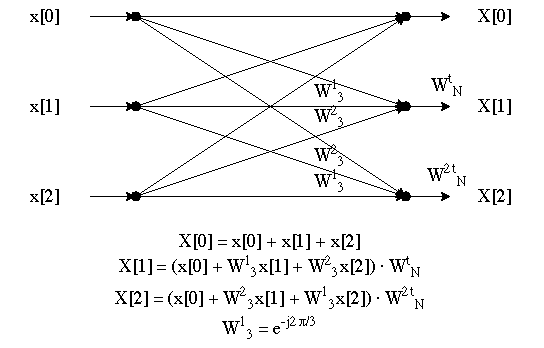
\includegraphics[width=0.8\textwidth]{figs/radix3_butterfly.pdf}
    \caption{Graphical representation of the radix-3 butterfly.}
    \label{fig:radix3_fft_diag}
\end{figure}

Similarly, changing $N_1$ to 5 leads to a radix-5 FFT algorithm. The coefficients then look like this:

\begin{align}
    X[k] &= \sum_{n=0}^{N/5-1} \bigl((x[n] + x[n + N/5] + x[n + 2N/5] \nonumber \\
    &\qquad + x[n + 3N/5] + x[n + 4N/5]) \cdot W_{N/5}^{nk}\bigr) \\
    X[k+N/5] &= \sum_{n=0}^{N/5-1} \bigl((x[n] + x[n + N/5]W_5^{1} + x[n + 2N/5]W_5^{2} \nonumber \\
    &\qquad + x[n + 3N/5]W_5^{3} + x[n + 4N/5]W_5^{4}) \cdot W_{N/5}^{nk}\bigr) \\
    X[k+2N/5] &= \sum_{n=0}^{N/5-1} \bigl((x[n] + x[n + N/5]W_5^{2} + x[n + 2N/5]W_5^{4} \nonumber \\
    &\qquad + x[n + 3N/5]W_5^{1} + x[n + 4N/5]W_5^{3}) \cdot W_{N/5}^{nk}\bigr) \\
    X[k+3N/5] &= \sum_{n=0}^{N/5-1} \bigl((x[n] + x[n + N/5]W_5^{3} + x[n + 2N/5]W_5^{1} \nonumber \\
    &\qquad + x[n + 3N/5]W_5^{4} + x[n + 4N/5]W_5^{2}) \cdot W_{N/5}^{nk}\bigr) \\
    X[k+4N/5] &= \sum_{n=0}^{N/5-1} \bigl((x[n] + x[n + N/5]W_5^{4} + x[n + 2N/5]W_5^{3} \nonumber \\
    &\qquad + x[n + 3N/5]W_5^{2} + x[n + 4N/5]W_5^{1}) \cdot W_{N/5}^{nk}\bigr)
\end{align}

The butterfly diagram for the radix-5 FFT algorithm can be represented as in Figure \ref{fig:radix5_fft_diag}.
\begin{figure}[htbp]
    \centering
    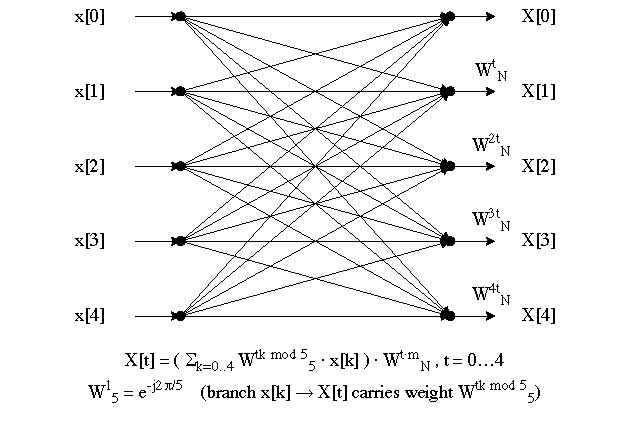
\includegraphics[width=0.9\textwidth]{figs/radix5_butterfly.pdf}
    \caption{Graphical representation of the radix-5 butterfly.}
    \label{fig:radix5_fft_diag}
\end{figure}

\subsection{Mixed-radix FFT}

When a non-power-of-two FFT length is required, the FFT can be implemented using a mixed-radix approach \cite{singleton1969}. This approach combines fixed-radix FFT algorithms (radix-2, radix-3, radix-5, etc.). The idea is to factor the FFT length $N$ into a product of prime factors $N = N_1 \times N_2 \times \cdots \times N_k$ and then use the fixed-radix FFT algorithms to compute the FFT. For example, if $N = 30$, we can factorize it into $N = 2 \times 3 \times 5$ and then use the radix-2, radix-3 and radix-5 FFT algorithms to compute the FFT.

The flowchart for the mixed-radix FFT algorithm on $N=30$ can be constructed step by step as follows. Decompose the whole calculation into three stages: radix-2, radix-3 and radix-5. The first stage is the radix-2 FFT algorithm as represented in Figure \ref{fig:n30_2x15}.

\begin{figure}[htbp]
    \centering
    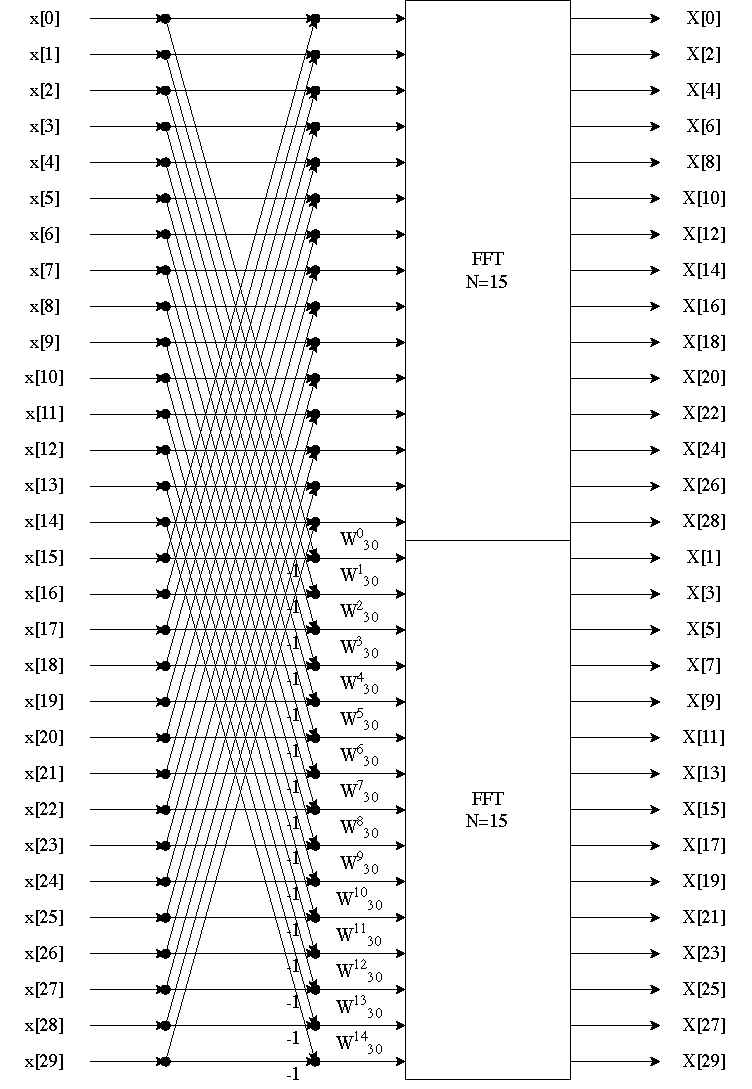
\includegraphics[width=1.0\textwidth]{figs/n30_2x15.pdf}
    \caption{Flowchart for the mixed-radix FFT algorithm on $N=30$.}
    \label{fig:n30_2x15}
\end{figure}

The remaining two DFTs of length 15 can then each be decomposed into two stages: radix-3 and radix-5. The first stage is the radix-3 FFT algorithm, as represented in Figure \ref{fig:n15_3x5}.

\begin{figure}[htbp]
    \centering
    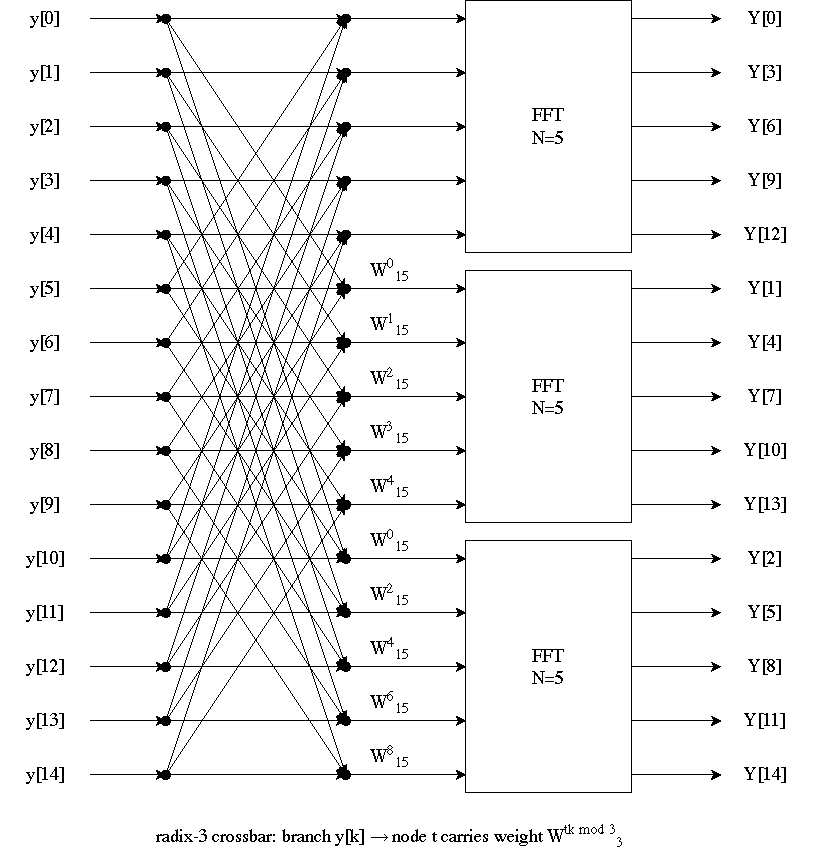
\includegraphics[width=1.0\textwidth]{figs/n15_3x5.pdf}
    \caption{Flowchart for the mixed-radix FFT algorithm on $N=30$.}
    \label{fig:n15_3x5}
\end{figure}

The $N=5$ stages are just radix-5 butterflies, as shown in Figure \ref{fig:radix5_fft_diag}.

So, the total flowchart for the mixed-radix FFT algorithm on $N=30$ can be represented as in Figure \ref{fig:n30_full_graph}.
\begin{figure}[htbp]
    \centering
    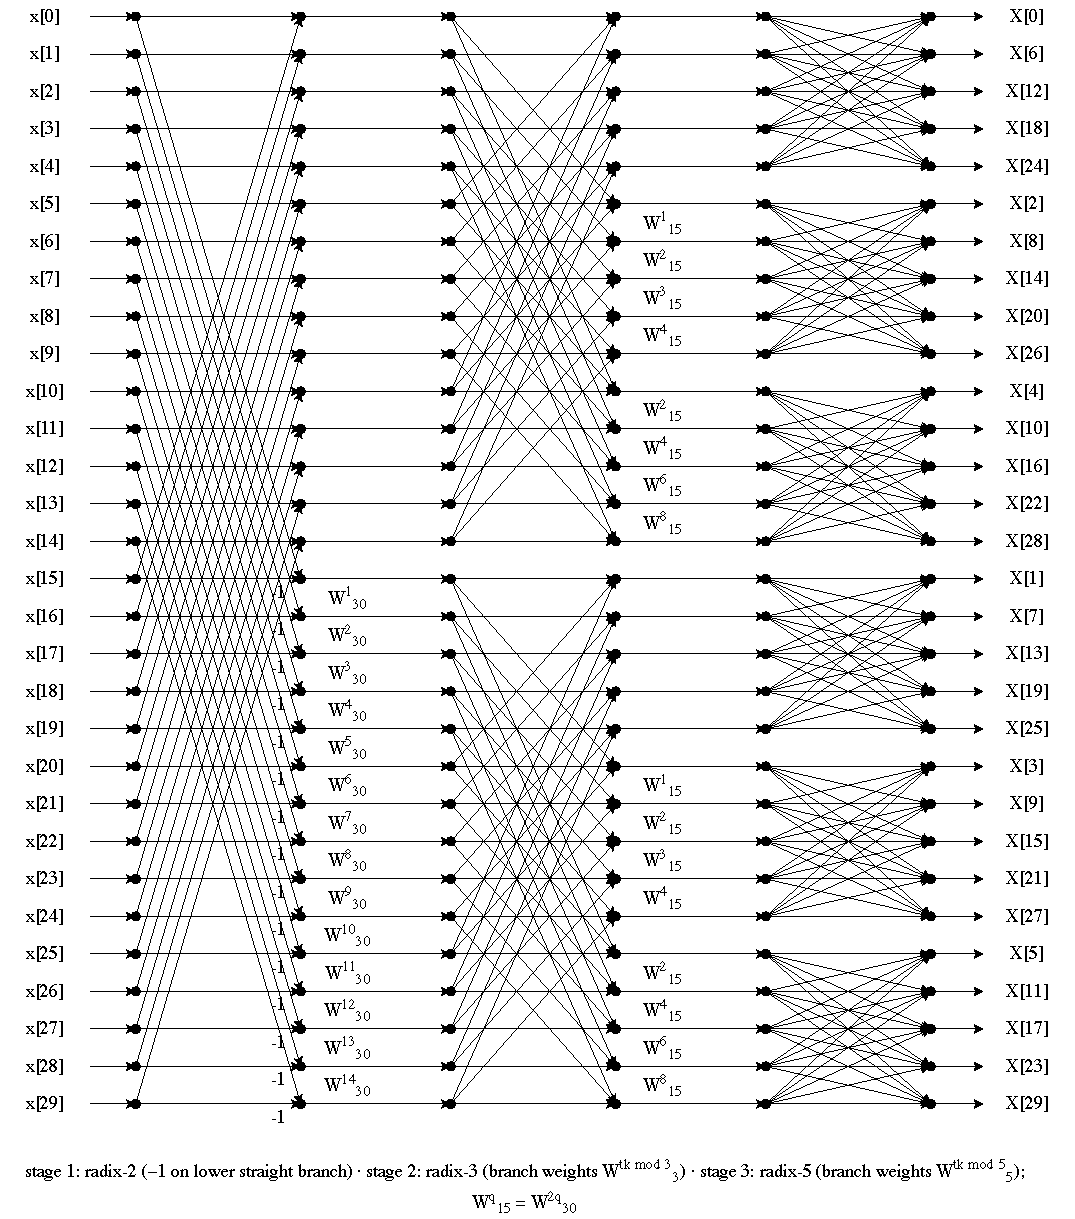
\includegraphics[width=1.0\textwidth]{figs/n3_full_graph.pdf}
    \caption{Flowchart for the mixed-radix FFT algorithm on $N=30$.}
    \label{fig:n30_full_graph}
\end{figure}

\subsection{Digit inversion}

The output samples of the DIF algorithm come in a scrambled order regardless of the length of the FFT. To get the samples in the correct order, digit inversion is required. Digit inversion is the process of reversing the order of the digits of a sample's index in the appropriate base number system.

The radix-2 FFT algorithm shows the simplest case of digit inversion. By inspecting the indices of the output samples in the full butterfly diagram for $N=8$ (Figure \ref{fig:radix2_fft_1_diag}), it can be seen that the indices are in the order 0, 4, 2, 6, 1, 5, 3, 7. In Table \ref{tab:radix2_fft_1_diag}, the indices are presented in the decimal and binary systems in the first two columns.

\begin{table}[H]
    \centering
    \begin{tabular}{|c|c|c|c|}
        \hline
        \textbf{Index} & \textbf{Binary} & \textbf{Inverted Binary} & \textbf{Inverted Decimal} \\
        \hline
        0 & 000 & 000 & 0 \\
        \hline
        4 & 100 & 001 & 1 \\
        \hline
        2 & 010 & 010 & 2 \\
        \hline
        6 & 110 & 011 & 3 \\
        \hline
        1 & 001 & 100 & 4 \\
        \hline
        5 & 101 & 101 & 5 \\
        \hline
        3 & 011 & 110 & 6 \\
        \hline
        7 & 111 & 111 & 7 \\
        \hline
    \end{tabular}
    \caption{Indices of output samples in the full butterfly diagram for $N=8$.}
    \label{tab:radix2_fft_1_diag}
\end{table}

By simply reversing the order of the digits of the index in the binary system, the inverted index in the decimal system is obtained.

A similar approach can be applied to the radix-3 and radix-5 FFT algorithms. They require digit inversion in the base-3 and base-5 number systems, respectively.

A more complex case is the mixed-radix FFT algorithm. It requires digit inversion in the base-2, base-3 and base-5 number systems together. The index is written in a mixed-radix positional system instead of binary, and then the digits are reversed together with the base of each digit.

Concretely, any index $n \in [0,N)$ can be written uniquely as:
\begin{equation}
    n = d_1 \cdot \frac{N}{r_1} + d_2 \cdot \frac{N}{r_1 r_2} + \cdots + d_{k-1} \cdot \frac{N}{r_1 r_2 \cdots r_{k-1}} + d_k \cdot 1, \quad d_i \in \{0, 1, \ldots, r_i - 1\},
\label{eq:mixed_radix_decomposition}
\end{equation}
where $d_i$ are the digits of the index $n$ in the mixed-radix positional system defined by the factorization $N = r_1 r_2 \cdots r_k$ into radices $r_i$. The digit-inverted index $\tilde{n}$ is then obtained by reversing the order of the digits, where the place values are now determined by the reversed sequence of radices $(r_k, r_{k-1}, \ldots, r_1)$:

\begin{equation}
    \tilde{n} = d_k \cdot \frac{N}{r_k} + d_{k-1} \cdot \frac{N}{r_k r_{k-1}} + \cdots + d_2 \cdot \frac{N}{r_k r_{k-1} \cdots r_2} + d_1 \cdot 1.
\label{eq:mixed_radix_inversion}
\end{equation}

As an example, consider $N = 15 = 5 \cdot 3$, i.e. $r_1 = 5$ and $r_2 = 3$. According to (\ref{eq:mixed_radix_decomposition}), an index $n$ is decomposed as $n = d_1 \cdot 3 + d_2$ with $d_1 \in \{0, 1, 2, 3, 4\}$ and $d_2 \in \{0, 1, 2\}$, and the digit-inverted index given by (\ref{eq:mixed_radix_inversion}) is $\tilde{n} = d_2 \cdot 5 + d_1$. The resulting permutation of all fifteen indices is shown in Table \ref{tab:mixed_radix_digit_inversion}.

\begin{table}[H]
    \centering
    \begin{tabular}{|c|c|c|c|}
        \hline
        \textbf{Index} & \textbf{Digits $(d_1, d_2)$} & \textbf{Inverted digits $(d_2, d_1)$} & \textbf{Inverted index $\tilde{n}$} \\
        \hline
        0 & (0, 0) & (0, 0) & 0 \\
        \hline
        1 & (0, 1) & (1, 0) & 5 \\
        \hline
        2 & (0, 2) & (2, 0) & 10 \\
        \hline
        3 & (1, 0) & (0, 1) & 1 \\
        \hline
        4 & (1, 1) & (1, 1) & 6 \\
        \hline
        5 & (1, 2) & (2, 1) & 11 \\
        \hline
        6 & (2, 0) & (0, 2) & 2 \\
        \hline
        7 & (2, 1) & (1, 2) & 7 \\
        \hline
        8 & (2, 2) & (2, 2) & 12 \\
        \hline
        9 & (3, 0) & (0, 3) & 3 \\
        \hline
        10 & (3, 1) & (1, 3) & 8 \\
        \hline
        11 & (3, 2) & (2, 3) & 13 \\
        \hline
        12 & (4, 0) & (0, 4) & 4 \\
        \hline
        13 & (4, 1) & (1, 4) & 9 \\
        \hline
        14 & (4, 2) & (2, 4) & 14 \\
        \hline
    \end{tabular}
    \caption{Digit inversion for the mixed-radix decomposition $N = 15 = 5 \cdot 3$.}
    \label{tab:mixed_radix_digit_inversion}
\end{table}

Note that the digits $(d_1, d_2)$ are read in bases $(5, 3)$, while the inverted digits $(d_2, d_1)$ are read in the reversed bases $(3, 5)$. The obtained permutation $(0, 5, 10, 1, 6, 11, 2, 7, 12, 3, 8, 13, 4, 9, 14)$ is exactly the order in which the output samples of the whole DIF FFT of length $N = 15$ appear: the first (radix-5) stage decimates the output indices into five groups according to $k \bmod 5$, i.e. $\{X[0], X[5], X[10]\}$, $\{X[1], X[6], X[11]\}$, and so on, while the final (radix-3) stage produces each group in natural order.

Digit inversion is an important step in the mixed-radix FFT algorithm, as it ensures that the output samples are in the correct order.

\section{Inverse FFT}

The forward DFT was discussed in the previous section. The inverse DFT is the inverse operation of the forward DFT and is defined as:
\begin{equation}
    x[n] = \frac{1}{N} \sum_{k=0}^{N-1} X[k] \cdot W_N^{-nk}
\end{equation}
where $W_N = e^{-j\frac{2\pi}{N}}$ is the twiddle factor.

The inverse DFT can be implemented using the same algorithm as the forward DFT in two ways:
\begin{itemize}
    \item swapping the real and imaginary parts of the input and output samples, or
    \item conjugating the input and output samples.
\end{itemize}
Both ways require a division by $N$ at the end of the algorithm.

Swapping and conjugating methods are represented in Figures \ref{fig:inverse_fft_swapping} and \ref{fig:inverse_fft_conjugating} respectively.
\begin{figure}[H]
    \centering
    \begin{subfigure}{\textwidth}
        \centering
        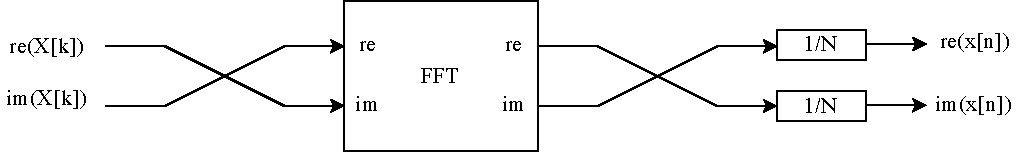
\includegraphics[width=0.9\textwidth]{figs/ifft_swap.pdf}
        \caption{Swapping method.}
        \label{fig:inverse_fft_swapping}
    \end{subfigure}

    \medskip

    \begin{subfigure}{\textwidth}
        \centering
        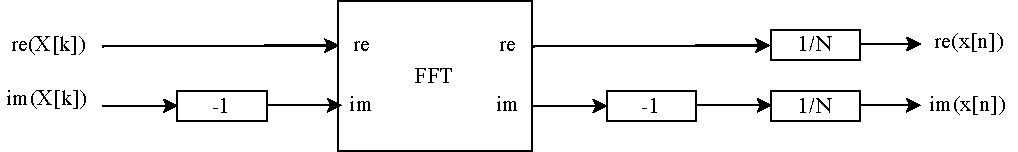
\includegraphics[width=0.9\textwidth]{figs/ifft_conjugate.pdf}
        \caption{Conjugating method.}
        \label{fig:inverse_fft_conjugating}
    \end{subfigure}
    \caption{Inverse DFT calculation using the forward FFT algorithm.}
    \label{fig:inverse_fft_methods}
\end{figure}
The conjugating method requires more hardware resources than the swapping method, because the negation of the imaginary part may need a full adder when it is represented in a fixed-point format (effectively two's complement). The swapping method requires only a swap of the two components.

\section{Fixed-point number representation}
\label{sec:fixed_point}

Hardware implementations of numerical algorithms often have a requirement to be resource-efficient and as fast as possible while maintaining good enough mathematical performance (such as the Signal-to-Noise Ratio, SNR). Floating-point arithmetic is not always the best choice due to its high compute latency and large resource footprint; the DSP blocks and block RAMs of an FPGA are integer resources, and floating-point operators built on top of them cost several times the logic and latency of their integer counterparts.
To achieve this, so-called fixed-point arithmetic is often used. It is a form of integer arithmetic that is used to represent real numbers in a fixed-precision format.

Fixed-point number representation can be illustrated as in Figure \ref{fig:fixed_point_representation}.

\begin{figure}[H]
    \centering
    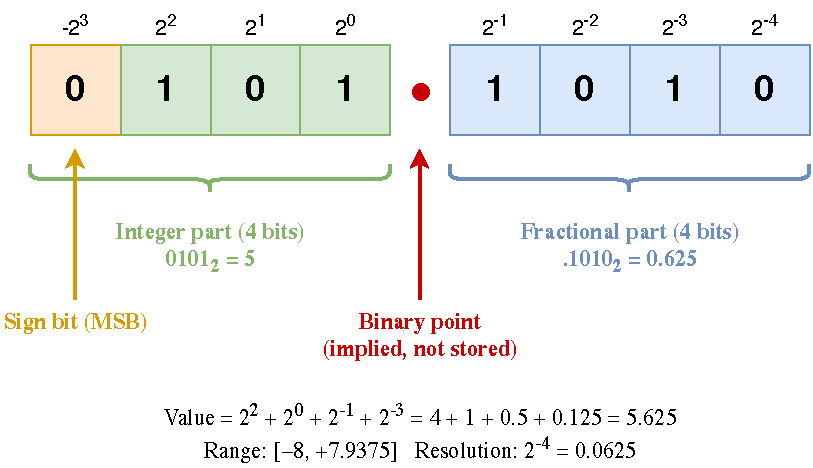
\includegraphics[width=0.9\textwidth]{figs/fixed_point_represente.pdf}
    \caption{Fixed-point representation — signed Q4.4, value = 5.625.}
    \label{fig:fixed_point_representation}
\end{figure}
It consists of a fixed number of bits for the integer part and a fixed number of bits for the fractional part. Between the integer and the fractional part there is an implied binary point. There is also a sign bit at the MSB position. The value of the fixed-point number is then given by the formula:
\begin{equation}
    value = \frac{integer}{2^fractional}
\end{equation}
where $integer$ is the integer part and $fractional$ is the fractional part.

The most interesting attribute of fixed-point number representation is that it allows a very efficient implementation of arithmetic operations using simple integer arithmetic.
For example, addition of two fixed-point numbers is equivalent to addition of two integers. Multiplication of two fixed-point numbers is equivalent to multiplication of two integers, with the caveat that the result is shifted by the number of fractional bits to fit into the fixed-point format. The shift is only a matter of which bits of the product are kept, so it costs nothing in hardware.

The handling of overflow and underflow is somewhat more complex. If the result of an arithmetic operation is too large to fit into the fixed-point format, it will overflow. If the result is too small to fit into the fixed-point format, it will underflow. These events are catastrophic for the mathematical performance of the algorithm, since they lead to strong spurs in the signal spectrum.
A logical step would be to grow the fixed-point format (increase the number of bits for the integer and fractional parts) to accommodate the result of the operation. This is fine if such bit growth is allowed by the resource constraints. But when this is not possible or not desirable, either a saturation mechanism or a scaling mechanism can be used. The saturation mechanism sets the result to the maximum or minimum value of the fixed-point format. The scaling mechanism scales the result by a factor that accommodates the bit growth of the operation, to the detriment of mathematical performance (some LSBs are discarded, so the SNR is degraded). Saturation needs a comparator and a multiplexer on every result and still distorts the signal when it triggers; scaling by a power of two is a plain shift and its noise is spread evenly over the spectrum, which is why scaling is the usual choice in FFT hardware and the one used in this design (Section \ref{sec:scaling}).

\chapter{Hardware Architecture}
\label{ch:hardware_architecture}
A high-performance FFT implementation is a must for telecommunication systems. A direct pipelined implementation of the mixed-radix FFT algorithm in hardware would be a translation of the diagram in Figure \ref{fig:n30_full_graph} into hardware. Data would have to be buffered between stages, where each stage would have $N$ inputs and $N$ outputs and process $N$ samples in each clock cycle.

This achieves the maximum possible throughput of the FFT algorithm and is implemented with $N$ complex adders and up to $N/2-1$ complex multipliers for the samples that need to be multiplied by non-trivial twiddle factors. The price is that every one of them is busy for only one clock cycle per frame; the rest of the time the hardware sits idle.

The first problem with this approach is that it requires an extremely large number of hardware resources to implement the complex adders and multipliers. Such a large design is barely feasible, or even impossible, to implement for the FFT sizes required for precoding in 5G, shown in Table \ref{tab:nr_precoding_sizes}.
The second problem is that all samples are required at the same time. That requires enough storage for $N$ samples between every two stages, and the storage has to be readable and writable in one cycle, which rules out block RAM and leaves only flip-flops.

To efficiently implement the mixed-radix FFT algorithm in hardware, a more efficient architecture is needed. The resource inventory of modern FPGAs includes blocks such as fast carry chains that implement fast adders, DSP blocks that implement pipelined multipliers and MAC units, and on-chip fast SRAM blocks (e.g. block RAM in Xilinx FPGAs). Efficient use of these blocks is the key to the success of the hardware implementation of any FPGA-based DSP algorithm, not just the mixed-radix FFT algorithm. The architecture therefore has to be chosen so that the multipliers land in DSP blocks, the buffers land in block RAM and the fabric is left with the control and the adders only.

\section{Streaming Mixed-Radix FFT Architecture}

The streaming mixed-radix FFT architectures are pipelined implementations of the mixed-radix FFT algorithm. They are designed to solve the resource utilization problem by processing samples sequentially. Commonly, they process one sample per clock cycle, but there are also architectures that process multiple samples per clock cycle. Streaming architectures reuse a single FFT butterfly per stage to process different samples sequentially, so the number of adders and multipliers grows with the number of stages, $\log_r N$, and not with $N$ itself. The throughput of one sample per cycle is exactly what an OFDM front-end delivers, so nothing is lost by the serialization.

The most common architectures are the Single-path Delay Feedback (SDF) and Multi-path Delay Feedback (MDF) architectures. This work focuses on the SDF architecture, which is also the basis of most of the reported non-power-of-two FFT designs \cite{bautista2023}.

\subsection{SDF Architecture}

The SDF architecture is one of the earliest pipelined FFT implementations, appearing in \cite{groginsky1970}. It is a pipelined implementation of the FFT algorithm that processes samples sequentially by using a single FFT butterfly per stage.

An SDF FFT is composed of $s$ stages that contain one input and one output each. The order of the samples at the input of the $i$-th stage is the order of the inputs of the $i$-th stage in the signal flow graph of the mixed-radix FFT algorithm, top to bottom. The output of the $i$-th stage is the input of the $(i+1)$-th stage. The architecture is shown in Figure \ref{fig:sdf_radix_r} for radix $R$ FFT, where $R$ is the radix of the FFT.

\begin{figure}[H]
    \centering
    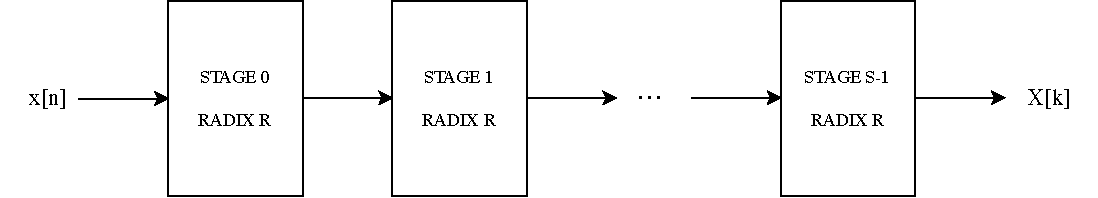
\includegraphics[width=1.0\textwidth]{figs/sdf_radix_r.pdf}
    \caption{SDF architecture for radix $R$ FFT.}
    \label{fig:sdf_radix_r}
\end{figure}

One stage of the SDF FFT architecture is shown in Figure \ref{fig:sdf_radix_r_stage}.

\begin{figure}[H]
    \centering
    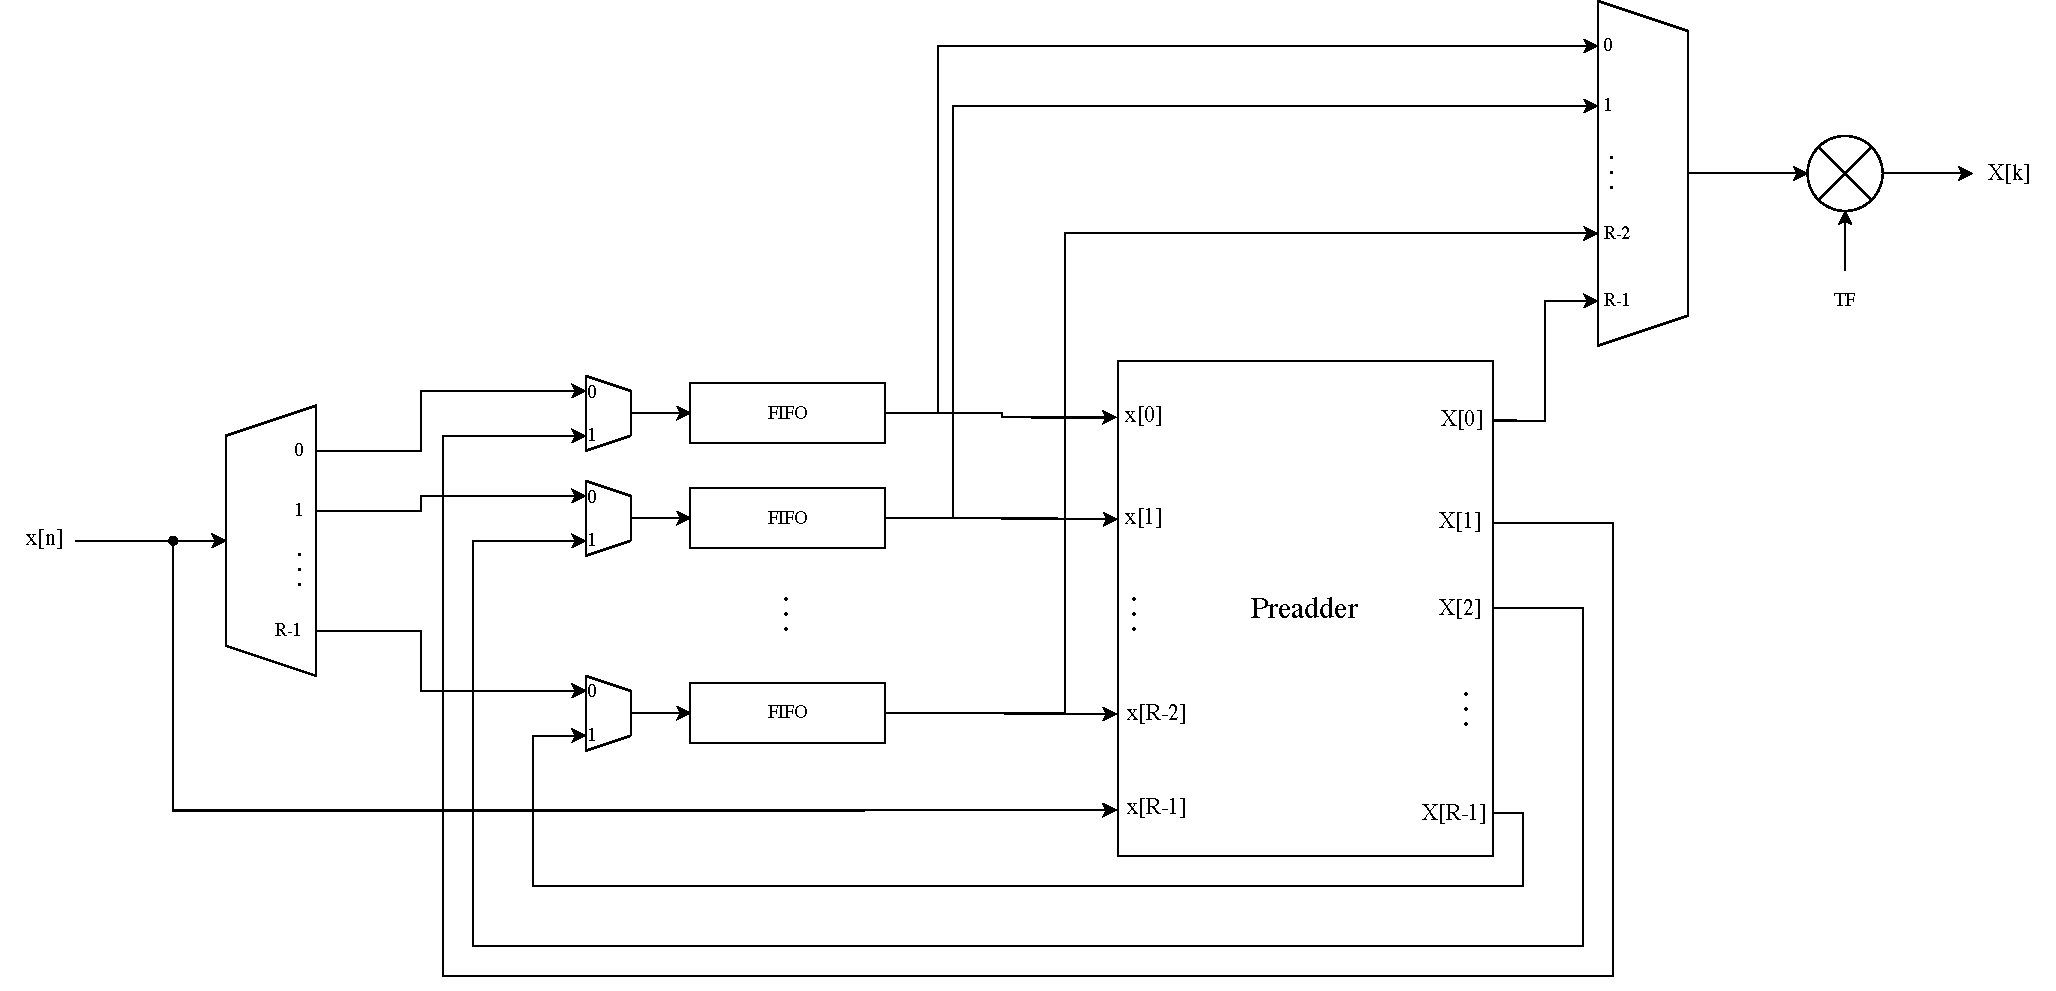
\includegraphics[width=1.0\textwidth]{figs/radix_r_stage.pdf}
    \caption{One stage of the SDF architecture for radix $R$ FFT.}
    \label{fig:sdf_radix_r_stage}
\end{figure}

The datapath of the stage consists of three main blocks: the FIFOs, a preadder and a rotator. The preadder performs the butterfly computations and is essentially a translation into hardware of the butterfly diagrams from the radix-2, radix-3 or radix-5 FFT algorithms, or from all of them combined in a reconfigurable manner, which will be discussed later. The rotator performs the twiddle factor multiplication and is a simple complex multiplier. The FIFOs are the only storage of the stage; everything else is arithmetic that maps onto adders and DSP blocks.

The idea of the SDF architecture is to process the samples sequentially with a single butterfly per stage. This requires the operations of a stage to be serialized onto a single butterfly and rotator. This is achieved by FIFOs that align the correct samples at the input of the preadder: the samples that belong to one butterfly arrive $N/r$ cycles apart, and the FIFOs hold the earlier ones until the last one arrives.

To illustrate the flow of the data stream and the need for FIFOs, consider the SDF architecture for a radix-2 FFT. The data flow is shown in Figure \ref{fig:sdf_buffer_flow_r2}.

\begin{figure}[H]
    \centering
    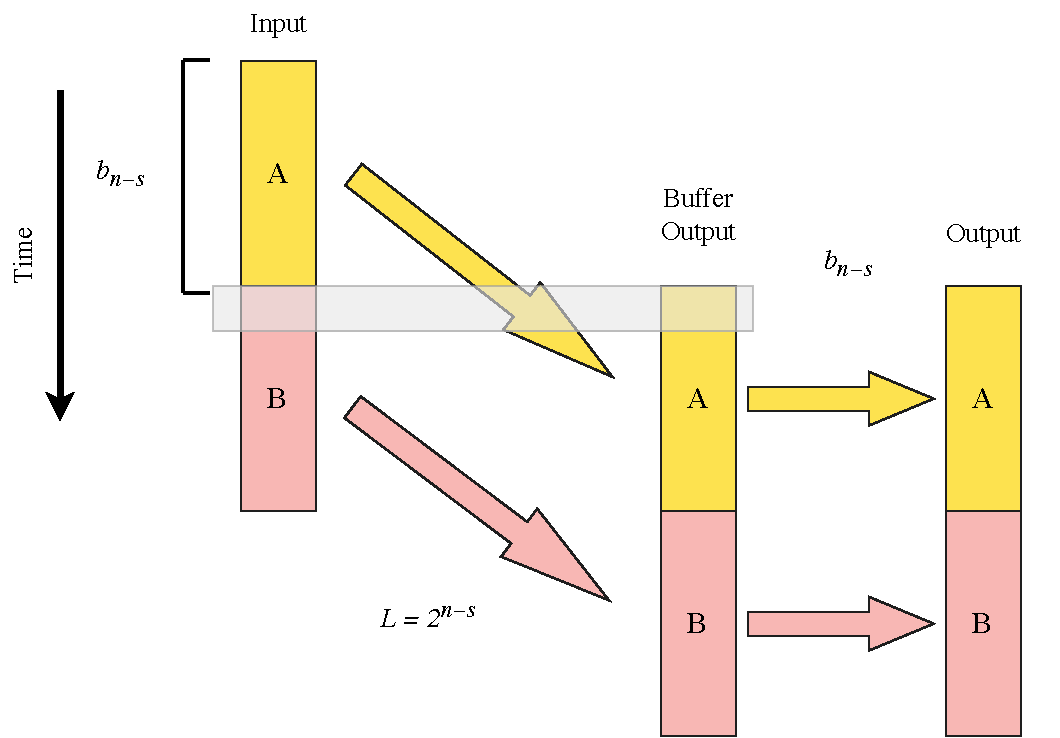
\includegraphics[width=0.80\textwidth]{figs/sdf_buffer_flow_r2.pdf}
    \caption{Data flow of the SDF architecture for radix-2 FFT.}
    \label{fig:sdf_buffer_flow_r2}
\end{figure}

It can be seen that, to perform the computation on the correct samples, a sample $x[n]$ needs to be aligned with the sample $x[n+N/2]$. This is achieved by the FIFO, which stores the incoming first half of the samples and reads them out when the second half of the samples starts arriving. This way, all samples $N/2$ apart are brought together into the preadder for the butterfly computation.

The radix-2 butterfly (Figure \ref{fig:radix2_fft_1_diag}) performs an addition and a subtraction of the input samples. With this architecture, the addition result of the preadder can be passed to the rotator right away, and the subtraction result (generated in the same cycle as the addition result) can be fed back to the FIFO and passed to the rotator when all the addition results have been generated. This is possible because the FIFO, full after the last sample of the first half of the samples is buffered, is read out as each new sample of the second half arrives. These FIFO reads make space each cycle for a new sample to be buffered, and since no input-sample buffering is needed yet (only the first half of the samples is buffered), the same FIFO can be used for both input and output. In other words, the FIFO is written and read in the same cycle during the second half, and the write-back of the subtraction result rides on the read of the delayed sample. The storage is therefore $N/2$ words for the whole stage, which is the minimum any architecture needs, since the first sample of the butterfly has to wait for the last one.

A radix-3 example of this data flow is shown in Figure \ref{fig:sdf_buffer_flow_r3}. Instead of buffering just the first half of the samples, it buffers the first two thirds of the samples in two separate FIFOs, each holding one of the thirds, and reads them out when the last third of the samples starts arriving. This way, all samples $N/3$ apart are brought together into the preadder for the butterfly computation. During the last third, the two FIFOs are read and, in the meantime, refilled with the two butterfly outputs that are not passed to the rotator right away. The same would be true for a radix-5 stage with four FIFOs of depth $N/5$.

\begin{figure}[H]
    \centering
    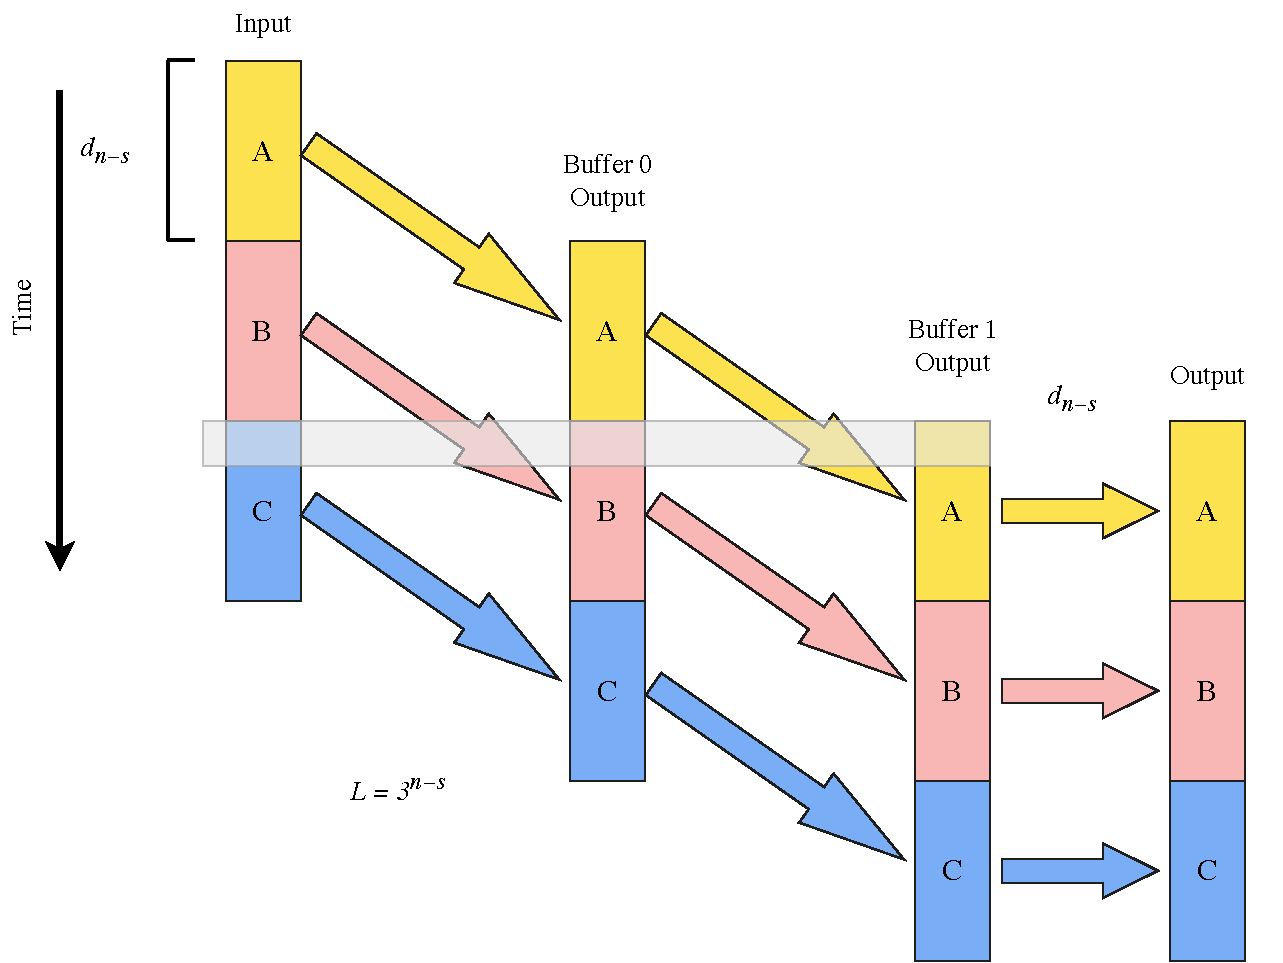
\includegraphics[width=0.95\textwidth]{figs/sdf_buffer_flow_r3.pdf}
    \caption{Data flow of the SDF architecture for radix-3 FFT.}
    \label{fig:sdf_buffer_flow_r3}
\end{figure}

The depth of the FIFOs is determined by the butterfly size. The butterfly size is the number of elementary butterfly operations in a stage. For example, for a radix-2 $N=2$ FFT, the butterfly size of its only stage is 1, so its FIFO depth is 1. For a radix-3 $N=9$ FFT, the butterfly size of its first stage (there are two stages in total) is 3, because it essentially performs 3 butterfly computations on 9 samples, so its FIFO depth is 3 for both FIFOs. The depth therefore shrinks by a factor of the radix from stage to stage, and the first stage alone holds $(r-1)/r$ of the total storage of the chain.

\section{Microarchitecture}

To fulfill the requirements of the 5G NR standard in the first place, all 53 FFT sizes need to be supported by the hardware implementation. Table \ref{tab:fft_sizes_factorized} presents the required FFT sizes factorized into the $2^i \cdot 3^j \cdot 5^k$ form. Reconfigurable architectures that cover such size sets with processing elements of changeable radix have been reported for the LTE and 5G sizes in \cite{shih2018, yang2023}; the stage described in this chapter follows the same idea of one datapath whose radix and delay are set by the configuration, built around the SDF structure.

\begin{table}[H]
\centering
\caption{The 53 required FFT sizes factorized as $N = 2^{i} \cdot 3^{j} \cdot 5^{k}$.}
\medskip
\label{tab:fft_sizes_factorized}
\begin{tabular}{c | c c c | c || c | c c c | c}
\hline
$N$ & $i$ & $j$ & $k$ & stages & $N$ & $i$ & $j$ & $k$ & stages\\
\hline
\hline
12 & 2 & 1 & 0 & 3 & 864 & 5 & 3 & 0 & 8\\
24 & 3 & 1 & 0 & 4 & 900 & 2 & 2 & 2 & 6\\
36 & 2 & 2 & 0 & 4 & 960 & 6 & 1 & 1 & 8\\
48 & 4 & 1 & 0 & 5 & 972 & 2 & 5 & 0 & 7\\
60 & 2 & 1 & 1 & 4 & 1080 & 3 & 3 & 1 & 7\\
72 & 3 & 2 & 0 & 5 & 1152 & 7 & 2 & 0 & 9\\
96 & 5 & 1 & 0 & 6 & 1200 & 4 & 1 & 2 & 7\\
108 & 2 & 3 & 0 & 5 & 1296 & 4 & 4 & 0 & 8\\
120 & 3 & 1 & 1 & 5 & 1440 & 5 & 2 & 1 & 8\\
144 & 4 & 2 & 0 & 6 & 1500 & 2 & 1 & 3 & 6\\
180 & 2 & 2 & 1 & 5 & 1536 & 9 & 1 & 0 & 10\\
192 & 6 & 1 & 0 & 7 & 1620 & 2 & 4 & 1 & 7\\
216 & 3 & 3 & 0 & 6 & 1728 & 6 & 3 & 0 & 9\\
240 & 4 & 1 & 1 & 6 & 1800 & 3 & 2 & 2 & 7\\
288 & 5 & 2 & 0 & 7 & 1920 & 7 & 1 & 1 & 9\\
300 & 2 & 1 & 2 & 5 & 1944 & 3 & 5 & 0 & 8\\
324 & 2 & 4 & 0 & 6 & 2160 & 4 & 3 & 1 & 8\\
360 & 3 & 2 & 1 & 6 & 2304 & 8 & 2 & 0 & 10\\
384 & 7 & 1 & 0 & 8 & 2400 & 5 & 1 & 2 & 8\\
432 & 4 & 3 & 0 & 7 & 2592 & 5 & 4 & 0 & 9\\
480 & 5 & 1 & 1 & 7 & 2700 & 2 & 3 & 2 & 7\\
540 & 2 & 3 & 1 & 6 & 2880 & 6 & 2 & 1 & 9\\
576 & 6 & 2 & 0 & 8 & 2916 & 2 & 6 & 0 & 8\\
600 & 3 & 1 & 2 & 6 & 3000 & 3 & 1 & 3 & 7\\
648 & 3 & 4 & 0 & 7 & 3072 & 10 & 1 & 0 & 11\\
720 & 4 & 2 & 1 & 7 & 3240 & 3 & 4 & 1 & 8\\
768 & 8 & 1 & 0 & 9 & & & & & \\
\hline
\end{tabular}
\end{table}

The number of radix-2, radix-3 and radix-5 stages needed to cover all FFT sizes is 10, 6 and 3, respectively. This means that the SDF architecture needs to support up to 10 radix-2 stages, 6 radix-3 stages and 3 radix-5 stages, but not all of them are active at the same time. The table tells, for every size, how many stages of each radix are needed; the maximum in every column, and not the sum, is what the hardware has to provide.
Implementing all of them at the same time would require a large amount of hardware resources, which is feasible but not optimal. Therefore, the SDF architecture is implemented in a reconfigurable manner, because not all of the stages are needed at the same time. In fact, the maximum number of stages active in one configuration is 11, for $N=3072$. If a stage can be reconfigured to be a radix-2 stage, a radix-3 stage or a radix-5 stage, or some needed combination of them, the hardware implementation can be optimized to use only the necessary number of stages. The reconfiguration is quasi-static: the FFT size changes when the carrier configuration changes, i.e. rarely, and never in the middle of a frame, so the radix of a stage can be treated as a constant while a frame is in flight.

This reconfigurable architecture leads to the high-level block diagram of the SDF architecture shown in Figure \ref{fig:sdf_reconfigurable_high_level}, where each stage is a reconfigurable block that can be configured as a radix-2 stage, a radix-2/3 stage or a radix-2/3/5 stage. If a stage is not needed, it can be bypassed by reconfiguring it to be in bypass mode. The order of the capabilities along the chain is not arbitrary: the radix-3 and radix-5 stages are placed where their FIFOs are the shallowest, so the storage that a radix-2/3/5 slot needs for its four delay FIFOs is kept small, while the first slots, which hold the deepest FIFOs, only ever have to be radix-2 capable.

\begin{figure}[H]
    \centering
    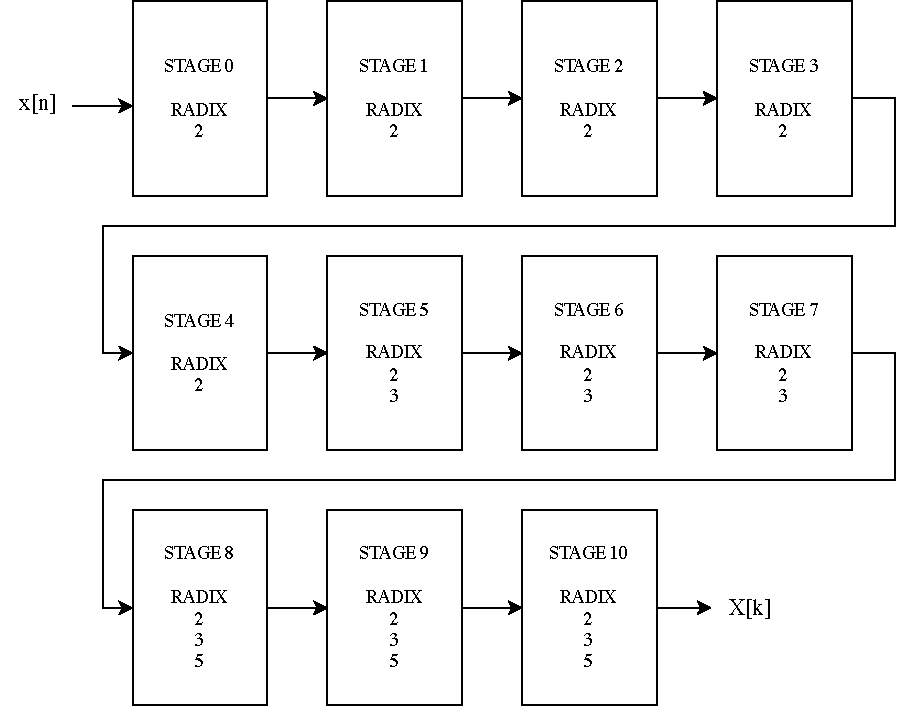
\includegraphics[width=0.9\textwidth]{figs/sdf_reconfig_high_level.pdf}
    \caption{High-level block diagram of the reconfigurable SDF architecture.}
    \label{fig:sdf_reconfigurable_high_level}
\end{figure}

So, three levels of stage capabilities are needed, each of them a superset of the previous one, so that a slot can always fall back to a lower radix or to bypass:
\begin{itemize}
    \item Radix-2 stage,
    \item Radix-2/3 stage,
    \item Radix-2/3/5 stage.
\end{itemize}

\subsection{Radix-2 Stage}

The proposed radix-2 stage is shown in Figure \ref{fig:sdf_reconfigurable_radix_2_stage}. Besides the FIFO, the preadder and the rotator, which were already discussed, it contains control logic responsible for the reconfiguration of the stage, a twiddle factor unit and another FIFO at the output.
The only role of the reconfiguration in this stage is to bypass the stage; the stage therefore carries no radix mode signals, only the bypass flag.
The twiddle factor unit is responsible for the generation of the twiddle factors for the stage when a certain FFT size is selected. It will be discussed in more detail in the next section.
All stages in the chain use the ready/valid protocol to communicate with each other. The rotator has a free-running pipeline inside it and a valid-bit shift register that marks which sample is valid. The pipeline cannot be stalled once a sample is issued into it, so the output skid FIFO plays the role of a skid buffer: it absorbs the valid samples that are already in flight in the rotator when the next stage is not ready to receive the data, and in the meantime the issue of new samples to the rotator is stopped. Another role of the skid FIFO is to buffer the samples when the stage is bypassed and no samples need to be processed. This cuts the combinational path for ready and valid signals between stages if the stage is bypassed, so a bypassed slot still re-registers the stream and does not lengthen the handshake path.

\begin{figure}[H]
    \centering
    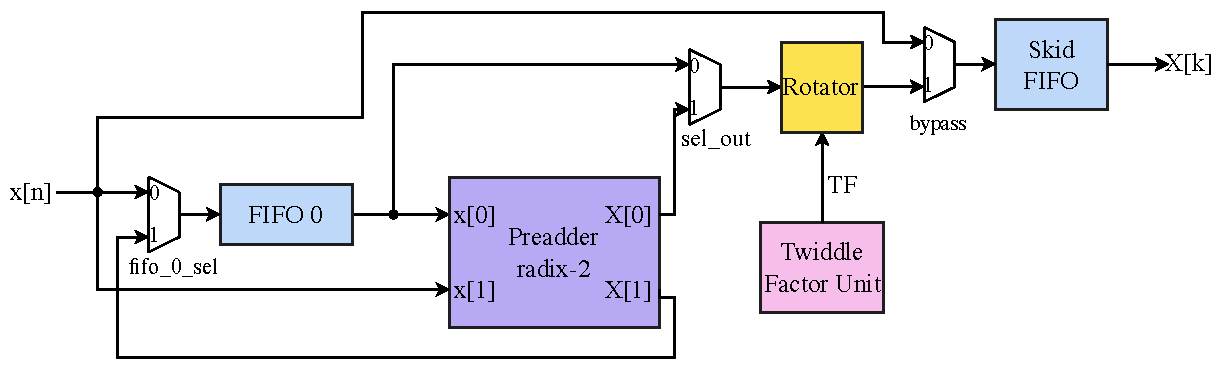
\includegraphics[width=1.0\textwidth]{figs/sdf_reconf_radix2_stage.pdf}
    \caption{Reconfigurable radix-2 stage of the SDF architecture.}
    \label{fig:sdf_reconfigurable_radix_2_stage}
\end{figure}

The preadder of the radix-2 stage is shown in Figure \ref{fig:radix_2_preadder}. It is a simple butterfly computation block that performs the addition and subtraction of the input samples and consists essentially of two signed adders. The block is purely combinational, so the results are available in the same cycle in which the inputs are read; this is the reason why the radix-2 stage needs no result FIFOs and writes the butterfly outputs straight back. Each output passes through a $\gg 1$ rnd block, which halves the result and rounds it back to the memory word; this is the scaling step of the stage and is described in Section \ref{sec:scaling}.

\begin{figure}[H]
    \centering
    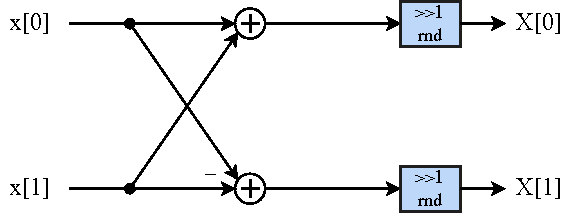
\includegraphics[width=0.5\textwidth]{figs/reconf2_bu_zola.pdf}
    \caption{Preadder of the radix-2 stage.}
    \label{fig:radix_2_preadder}
\end{figure}

\subsection{Radix-2/3 Stage}

The proposed radix-2/3 stage is shown in Figure \ref{fig:sdf_reconfigurable_radix_2_3_stage}. Besides the components also present in the radix-2 stage, it contains additional result FIFOs at the preadder outputs, whose role is explained below. The control logic now also drives the radix mode signals of the preadder and qualifies the second delay FIFO, which is only used in the radix-3 mode.

\begin{figure}[H]
    \centering
    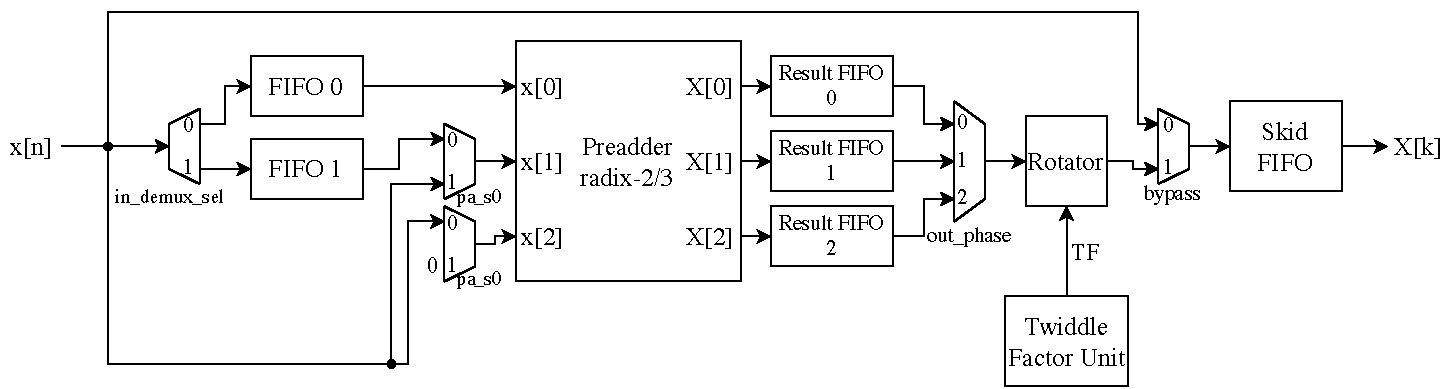
\includegraphics[width=1.0\textwidth]{figs/sdf_reconf_radix23_stage.pdf}
    \caption{Reconfigurable radix-2/3 stage of the SDF architecture.}
    \label{fig:sdf_reconfigurable_radix_2_3_stage}
\end{figure}

The radix-2/3 preadder is shown in Figure \ref{fig:radix_2_3_preadder}. It is a more complex butterfly computation block that, besides multiple additions and subtractions, also performs two multiplications by fixed coefficients. One of the coefficients is either $1$ or $0.5$, depending on the stage radix configuration. Since both values are powers of two, this "multiplication" does not require a multiplier at all -- it is implemented as a multiplexed arithmetic shift, which costs only a few multiplexers. The other coefficient is

\begin{equation}
    k_6 = -\sin\frac{2\pi}{3} = \frac{j}{2}\left(W_3^{-1} - W_3^{1}\right) = -\frac{\sqrt{3}}{2} \approx -0.8660,
\label{eq:coeff_k6}
\end{equation}

which is simply the imaginary part of the radix-3 twiddle factor $W_3 = -\frac{1}{2} - j\frac{\sqrt{3}}{2}$. Note that $k_6$ is a purely real number. This is the property that the Winograd-based radix-3 and radix-5 butterflies of \cite{qureshi2013} and the LTE kernels of \cite{lofgren2011} rely on: with the right grouping of the inputs, every coefficient of the 3- and 5-point DFT is either purely real or purely imaginary. A general complex multiplication $(a + jb)(c + jd)$ costs four real multiplications and two additions, but multiplying a complex sample by a purely real coefficient $k$ reduces to $k a + j k b$, which is only two real multiplications and no additions. The remaining factor $j$ that completes the radix-3 butterfly is pulled out of the coefficient and applied separately in the $j$ block of Figure \ref{fig:radix_2_3_preadder}: multiplication by $j$ is just a swap of the real and imaginary parts with one negation, so it costs a bit vector inversion and an adder in hardware (negation in two's complement is a bit inversion and addition of 1). The multiplier itself therefore only ever sees a real coefficient and maps onto two DSP blocks.

\begin{figure}[H]
    \centering
    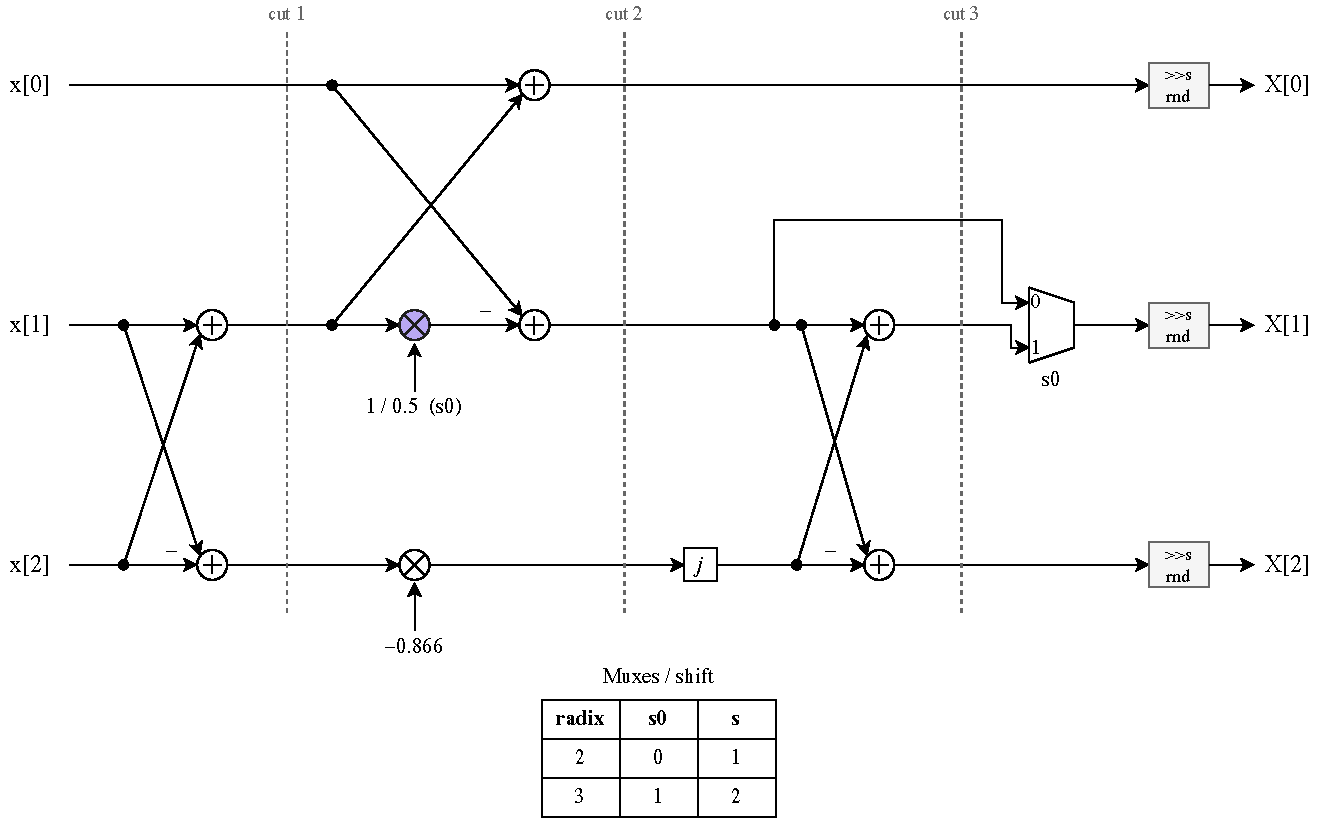
\includegraphics[width=1.0\textwidth]{figs/reconf23_bu_zola.pdf}
    \caption{Radix-2/3 preadder.}
    \label{fig:radix_2_3_preadder}
\end{figure}

Dashed vertical lines indicate the pipeline stages inserted to cut long combinational paths through the preadder. The cuts are placed so that the operand, product and rounding registers are absorbed into the DSP blocks, and the remaining adder levels are separated so that no path spans more than one adder level. This adds three clock cycles of latency to the stage, but it is necessary to achieve the desired maximum clock frequency. The introduced latency creates a data hazard that is resolved by the addition of the result FIFOs. If the direct write-back to the input FIFOs is considered with a preadder that has a latency of one or more clock cycles, for example 2 clock cycles, the following hazard scenario would occur:
\begin{itemize}
    \item Currently, the last third of the samples is being processed by the preadder.
    \item The last three samples for the calculation are passed to the preadder inputs.
    \item Because of the latency of the preadder, the three samples are not available at the preadder outputs in the same clock cycle, so they cannot be written back to the input FIFOs.
    \item In the next clock cycle, the first sample of the new stream of samples arrives at the first input FIFO, and the FIFO is written with new samples even though not all samples from the previous stream have been written back to it yet.
    \item After two clock cycles, the three samples are available at the preadder outputs and can be written back to the input FIFOs.
    \item The new stream of samples overlaps with the previous stream, and the samples are lost.
\end{itemize}
This would cause a data hazard because some samples are lost. This is resolved either by gating the new stream of samples, which creates bubbles and therefore lowers the throughput, or by adding a new set of FIFOs at the preadder outputs (with a depth equal to the depth of the input FIFOs plus the pipeline depth of the preadder, to accommodate the latency, like the skid FIFO does for the rotator output) to accept the preadder results. The result FIFOs are then read and the samples are passed to the rotator pipeline for twiddle factor multiplication. The price is a doubling of the storage of the stage, but in return the input side never has to stall on the preadder latency, and the input and output flows of the stage are decoupled (Section \ref{sec:flow_control}). The second option is therefore chosen.

The table below the preadder diagram shows the multiplexer select values for each of the radix configurations, together with the scaling shift $s$ applied in the $\gg s$ rnd blocks at the outputs: one bit in the radix-2 mode and two bits in the radix-3 mode (Section \ref{sec:scaling}). All select signals are derived from the quasi-static radix configuration, so they are registered once and do not change during a frame.


\subsection{Radix-2/3/5 Stage}

The proposed radix-2/3/5 stage is shown in Figure \ref{fig:sdf_reconfigurable_radix_2_3_5_stage}. Structurally it is the radix-2/3 stage with two more delay FIFOs and two more result FIFOs; the control logic qualifies the FIFOs that belong to the selected radix and holds the rest inactive, so in the radix-2 mode the stage behaves exactly like the radix-2 stage, only with a longer preadder pipeline.

\begin{figure}[H]
    \centering
    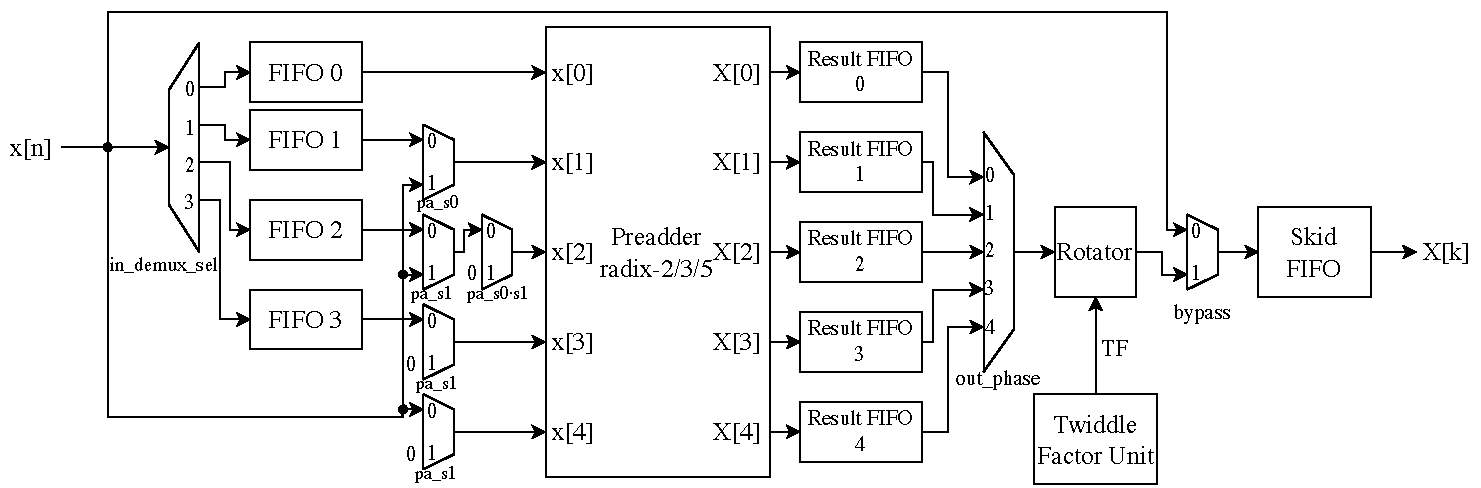
\includegraphics[width=1.0\textwidth]{figs/sdf_reconf_radix235_stage.pdf}
    \caption{Reconfigurable radix-2/3/5 stage of the SDF architecture.}
    \label{fig:sdf_reconfigurable_radix_2_3_5_stage}
\end{figure}

The radix-2/3/5 preadder is shown in Figure \ref{fig:radix_2_3_5_preadder}. It extends the radix-2/3 structure with the adder levels and coefficient multipliers required by the radix-5 butterfly. The multiplexed shift coefficient now takes the values $1$, $0.5$ or $0.25$ (again implemented as a shift), the shared multiplier selects between $k_6$ for the radix-3 mode and $k_2$ for the radix-5 mode, and three additional fixed multipliers apply the coefficients $k_3$, $k_4$ and $k_5$. Expressed both trigonometrically and through the twiddle factors $W_5^{k}$, the coefficients are:

\begin{align}
    k_2 &= \frac{1}{2}\left(\cos\frac{2\pi}{5} - \cos\frac{4\pi}{5}\right)
         = \frac{1}{4}\left(W_5^{1} + W_5^{-1} - W_5^{2} - W_5^{-2}\right)
         = \frac{\sqrt{5}}{4} \approx 0.5590, \\
    k_3 &= j\left(\sin\frac{4\pi}{5} - \sin\frac{2\pi}{5}\right)
         = \frac{1}{2}\left(W_5^{1} - W_5^{-1} - W_5^{2} + W_5^{-2}\right)
         \approx -j\,0.3633, \\
    k_4 &= -j\sin\frac{4\pi}{5}
         = \frac{1}{2}\left(W_5^{2} - W_5^{-2}\right)
         \approx -j\,0.5878, \\
    k_5 &= j\left(\sin\frac{2\pi}{5} + \sin\frac{4\pi}{5}\right)
         = \frac{1}{2}\left(W_5^{-1} - W_5^{1} + W_5^{-2} - W_5^{2}\right)
         \approx j\,1.5388.
\label{eq:coeffs_radix5}
\end{align}

These coefficients arise from the symmetries of the radix-5 twiddle factors: the real parts of $W_5^{k}$ and $W_5^{-k}$ are equal while their imaginary parts are opposite, which allows the DFT matrix to be factored into sums and differences of the inputs multiplied by the purely real combination $k_2$ and the purely imaginary combinations $k_3$, $k_4$ and $k_5$.

Note that every coefficient is again either purely real ($k_2$, $k_6$) or purely imaginary ($k_3$, $k_4$, $k_5$), so by the argument given for the radix-2/3 preadder each of the four coefficient multipliers costs only two real multiplications instead of four, mapping to eight real multipliers (DSP blocks) instead of sixteen. For $k_3$, $k_4$ and $k_5$ the zero real part is simply pruned by synthesis, while on the shared $k_6/k_2$ multiplier the factor $j$ needed in the radix-3 mode is applied structurally by the multiplexed $j$ block. Sharing this multiplier between the two modes is what keeps the radix-2/3/5 preadder at eight DSP blocks; a separate $k_6$ path would cost two more for a coefficient that is never used at the same time as $k_2$.

\begin{figure}[H]
    \centering
    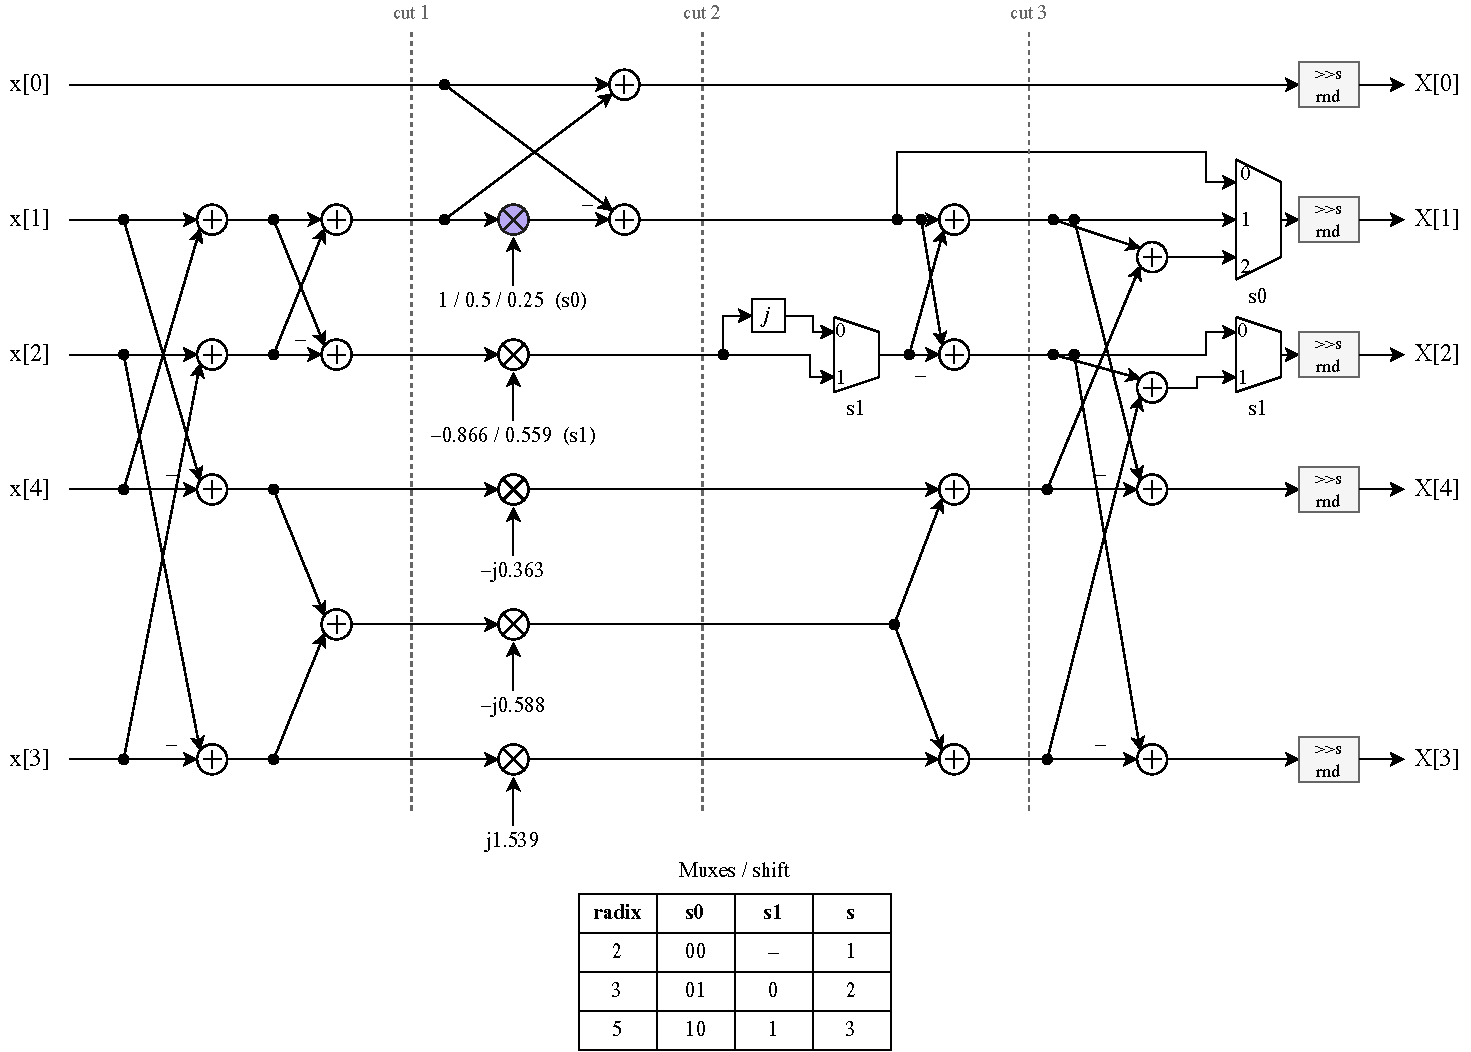
\includegraphics[width=1.0\textwidth]{figs/reconf235_bu_zola.pdf}
    \caption{Radix-2/3/5 preadder.}
    \label{fig:radix_2_3_5_preadder}
\end{figure}

Dashed vertical lines indicate the pipeline stages inserted to cut long combinational paths through the preadder. This adds three clock cycles of latency to the stage just like in the radix-2/3 case; the additional adder level of the radix-5 butterfly is absorbed into the existing cuts, so the latency does not grow with the capability.

The table below the preadder diagram shows the multiplexer select values for each of the radix configurations and the scaling shift $s$ of the output $\gg s$ rnd blocks: one, two or three bits for the radix-2, radix-3 and radix-5 modes. The shift amount is selected by the same \texttt{s0} signal that selects the radix mode, so the scaling rides on the existing mode decode and needs no control of its own.

\subsection{Twiddle Factor Unit}

The twiddle factor unit generates one twiddle factor for every output beat of the stage. Its block diagram is shown in Figure \ref{fig:twiddle_factor_unit}.

\begin{figure}[H]
    \centering
    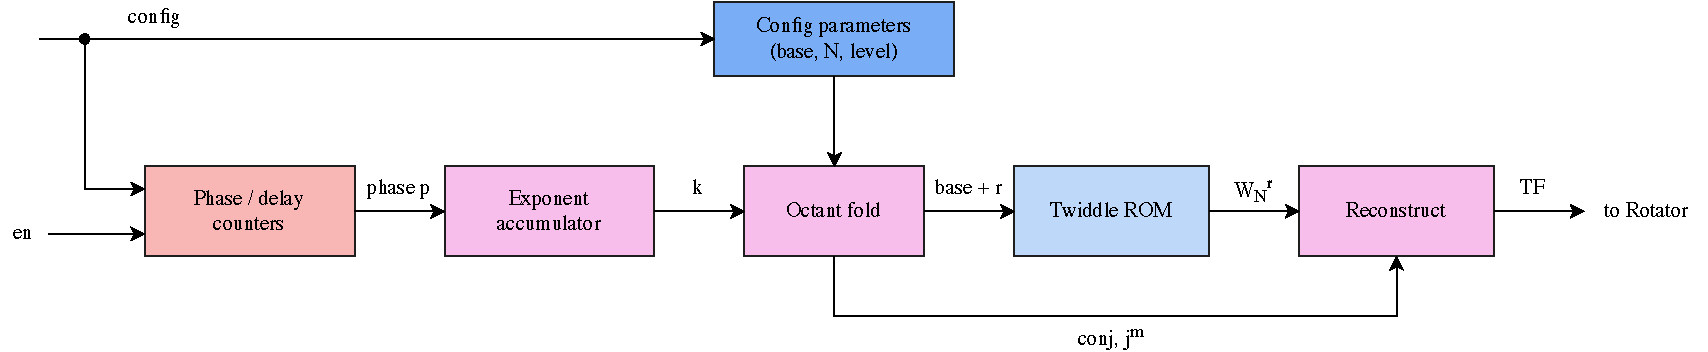
\includegraphics[width=1.0\textwidth]{figs/twiddle_factor_unit.pdf}
    \caption{Twiddle factor unit.}
    \label{fig:twiddle_factor_unit}
\end{figure}

The phase and delay counters (discussed in Section \ref{sec:phase_delay_counters}) track the output arm $p$ (which "arm" of the preadder result FIFOs the sample comes from) and the position $n$ inside the block (the index of the sample inside the arm block). From them the twiddle exponent $k = p \cdot n$ is formed by the exponent accumulator: it is cleared at the start of every block and incremented by $p$ on every beat, so no multiplier is needed. The accumulator is driven by the output beat, so it stalls together with the output flow and the exponent always stays aligned with the sample.

The twiddle factors are read from a ROM. Storing all $N$ points of the unit circle would be wasteful, so only the first octant ($0 \le r \le N/8$) is stored and the symmetry of the unit circle is used for the rest. The octant fold block reduces the exponent $k$ to the stored index $r$ in three steps (half, quarter and octant of the circle); each step sets a flag: a conjugate flag and a two-bit code $m$ of the unit multiplier $j^m$. The tables for all FFT sizes supported by the stage are packed into a single ROM, and the configuration parameters block supplies the base address and size $N$ of the selected configuration. The ROM is read synchronously, so it maps to block RAM and costs no fabric logic; the reconfiguration of the unit therefore reduces to a change of the base address and of the fold thresholds.

The flags travel alongside the ROM and are applied in the reconstruct block: the conjugate flag negates the imaginary part and the multiplication by $j^m$ is a swap and negation of the components, so the reconstruction is done only with multiplexers. All blocks of the unit are registered and the stage delays the data samples by the same number of cycles, so each twiddle factor meets its sample at the rotator input.

\subsection{Rotator}

The rotator multiplies every output sample of the stage by the twiddle factor supplied by the twiddle factor unit. Its structure is shown in Figure \ref{fig:rotator_unit}.

\begin{figure}[H]
    \centering
    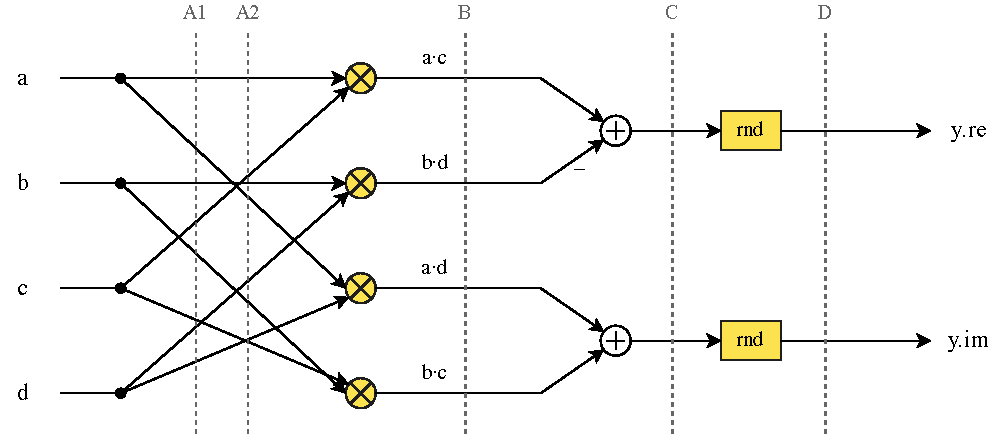
\includegraphics[width=0.9\textwidth]{figs/rotator_unit.pdf}
    \caption{Rotator.}
    \label{fig:rotator_unit}
\end{figure}

Unlike the preadder coefficients, the twiddle factor is a general complex number, so the full complex product is needed. With the sample $x = a + jb$ and the twiddle factor $W = c + jd$, the result is formed as $y = (ac - bd) + j(ad + bc)$, which takes four real multiplications and two additions. A three-multiplier form would save one DSP block per stage, but at the price of three extra adders in front of the multipliers and a longer critical path; since the DSP blocks are not the limiting resource of the design, the plain four-multiplier form is used. The products and their sums are kept in full precision; the result is quantized back to the memory word only once, in the rnd blocks, with half-up rounding.

The rotator is pipelined with five register cuts, marked with dashed lines in Figure \ref{fig:rotator_unit}: two operand registers (A1, A2), the product registers (B), the sum registers (C) and the rounding registers (D). The cuts are placed so that synthesis absorbs A1/A2, B and C into the input, multiplier and output registers of the four DSP blocks. A valid flag is delayed through the same number of registers, so the datapath runs freely without enables; whatever is in the pipeline is either a valid sample or invalid data that the flag tells the skid FIFO to ignore.

\subsection{Scaling and Rounding}
\label{sec:scaling}

All samples stored or streamed in the design -- in the delay, result and skid FIFOs and on the links between the stages -- share one fixed-point memory word. A butterfly, however, grows the signal: a radix-$r$ butterfly sums $r$ inputs, so its outputs can be up to $r$ times larger than the inputs. Without a countermeasure the word would overflow after a few stages. Growing the word by $\log_2 r$ bits in every stage would avoid the overflow, but it would make every FIFO, adder and multiplier downstream wider, and the FIFOs dominate the memory of the design.

Instead, the stages apply a fixed scaling schedule: every stage divides its butterfly outputs by a power of two that covers the growth of its radix, i.e. by $2^{s}$ with $s = \lceil \log_2 r \rceil$ -- one bit for radix-2, two bits for radix-3 and three bits for radix-5. A power of two is chosen deliberately, because dividing by three or five exactly would need a multiplier per output, while a division by $2^{s}$ is an arithmetic right shift, which costs no logic at all. The shift amount is selected by the same radix mode signal \texttt{s0} that configures the preadder. Since the shift always covers the growth, the stage output fits back into the memory word by construction and no saturation logic is needed. The price is the one already discussed in Section \ref{sec:fixed_point}: the bits shifted out are lost, so a small amount of quantization noise is added in every stage.

To keep this noise as low as possible, the arithmetic inside the preadder is done in a wider word and without intermediate rounding: the adder tree, the algorithmic $1/2$ and $1/4$ shifts of the radix-3 and radix-5 butterflies and the sums of the coefficient products are computed exactly, and only the coefficient products themselves are trimmed once on the post-adder of the DSP block. The scaling shift and the return to the memory word are then fused into a single operation at the exit of the preadder, the $\gg s$ rnd blocks in Figures \ref{fig:radix_2_preadder}, \ref{fig:radix_2_3_preadder} and \ref{fig:radix_2_3_5_preadder}: half of an output LSB is added, the word is shifted right by $s$ bits and truncated, which gives half-up rounding for free. In this way each stage rounds its data exactly once in the butterfly. The rotator adds a second rounding per stage, but no scaling: the magnitude of a twiddle factor is at most one, so the product needs no extra headroom and is only rounded back to the memory word, as described above.

Because the shift is $\lceil \log_2 r \rceil$ rather than $\log_2 r$, the radix-3 and radix-5 stages divide by four and eight instead of by three and five. After $n_2$ radix-2, $n_3$ radix-3 and $n_5$ radix-5 stages, the chain therefore delivers

\begin{equation}
    X'_k = X_k \cdot 2^{-S}, \qquad S = n_2 + 2 n_3 + 3 n_5,
\end{equation}

instead of the $X_k / N$ convention. The residual gain between the two is corrected by the final scaler at the end of the chain (Figure \ref{fig:top_level_control}), which multiplies every output by

\begin{equation}
    c = \frac{2^{S}}{N} = \left(\frac{4}{3}\right)^{n_3} \left(\frac{8}{5}\right)^{n_5},
\end{equation}

a real constant between $4/3$ and about $5.7$ for the supported sizes. The constant is computed for every configuration at elaboration time and selected together with the configuration at commit through the \texttt{SCALE} register. Correcting the gain once at the end of the chain is much cheaper than dividing exactly in every stage: since $c$ is real, the scaler needs only one real multiplication per component (one DSP block each), the half-up rounding constant again rides on the post-adder, and the product is rounded once to the memory word. The scaler is a three-stage pipeline with the same credit-gated output skid as the stage, so the output of the core is delivered as $X_k / N$ with a registered handshake.

\subsection{FIFOs}

All buffers of the stage -- the delay FIFOs, the result FIFOs and the output skid -- are instances of one show-ahead FIFO. The read port always presents the oldest word together with a valid flag, and the read enable pops it; the consuming side can therefore inspect the word first and decide cycle by cycle whether to take it, which is exactly what the drain gate and the output handshake need.

The storage is a simple dual-port block RAM with one write port and one read port. Two ports are required because in streaming operation the FIFO is written and read in the same cycle: while the joint phase pops one sample per delay FIFO, the fill phases of the next block are already writing new samples into them. The synchronous read of the block RAM has a latency of two cycles (memory read plus the RAM output register), so two additional fabric registers are placed in front of the read port. They hold the two oldest words, are refilled from the RAM in the background, and make back-to-back pops run at one word per cycle without bubbles; when the RAM is empty, writes bypass directly into these registers, so the FIFO also works as a delay line of depth one.

The reconfigurability of the depth costs nothing in the FIFO itself. Each FIFO is built at elaboration time for the largest configuration of its slot (depth $N_{max}/r$ for the delay FIFOs), and the effective depth at runtime is set purely by occupancy: for a smaller FFT size the control simply writes fewer words ($N/r$ for the selected configuration) before the joint phase starts popping them, so the same RAM acts as a shorter delay line. The upper part of the RAM is simply never visited. Only the delay compare value in the counters changes between configurations; the read and write pointers wrap at the physical depth, which does not need to be a power of two.

\subsection{Phase and Delay Counters}

\label{sec:phase_delay_counters}
All timing inside a stage is derived from one pair of cascaded counters, shown in Figure \ref{fig:phase_delay_counters}. The delay counter $n$ advances on every beat and counts the position of the sample inside the current block, $0 \ldots D-1$, where $D = N/r$ is the delay of the stage for the selected configuration. When it wraps, the phase counter $p$ advances by one; $p$ counts the block, i.e. the arm of the butterfly the sample belongs to, $0 \ldots r-1$, and wraps at the radix. The beat is therefore mapped to the pair $(p, n)$, as illustrated by the example at the bottom of the figure.

\begin{figure}[H]
    \centering
    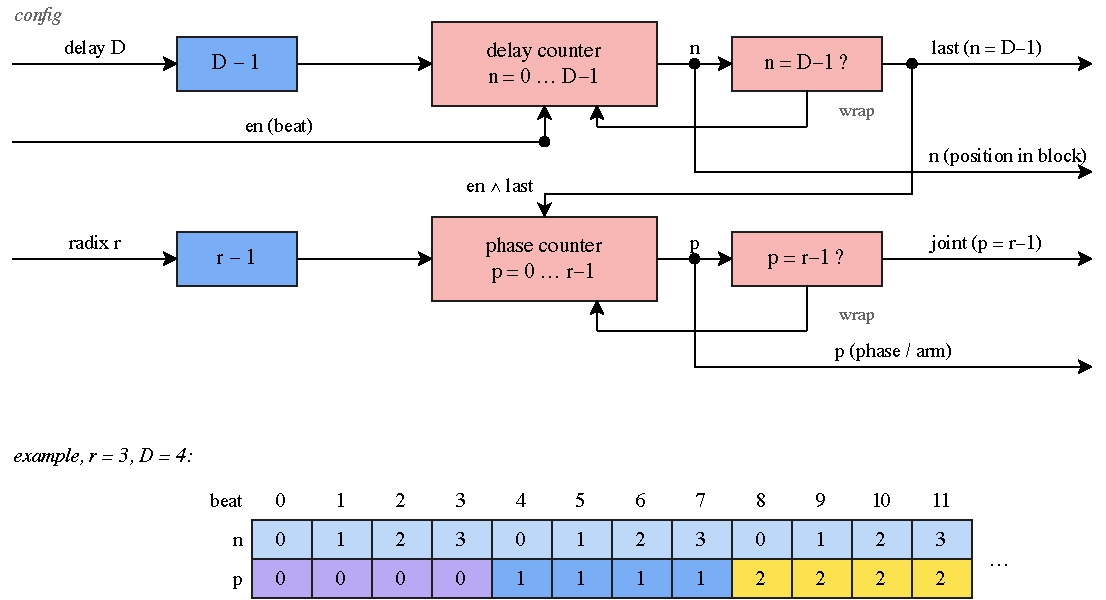
\includegraphics[width=0.95\textwidth]{figs/phase_delay_counters.pdf}
    \caption{Phase and delay counters.}
    \label{fig:phase_delay_counters}
\end{figure}

The two compare values $D-1$ and $r-1$ are the only inputs that depend on the configuration. They are registered once from the quasi-static configuration, so the per-beat wrap compares start from flip-flops and no subtractor sits on the counting path. The comparator outputs are exported as flags: \texttt{last} marks the final sample of a block and \texttt{joint} marks the final phase, in which the preadder is fed and the result FIFOs are written. Everything else in the stage -- FIFO enables, multiplexer selects, the twiddle exponent -- is derived from these two counters and two flags, so the whole stage sequencing costs a handful of flip-flops and two comparators.

Every stage contains two instances of this counter pair, one enabled by the input beats and one by the output beats. The input pair steers the input demultiplexer and the FIFO write enables and defines the joint phase; the output pair steers the output multiplexer and supplies $p$ and $n$ to the twiddle factor unit, which forms the exponent $k = p \cdot n$ from them. Because the two pairs run independently, the input and output sides of the stage are decoupled, as described in Section \ref{sec:flow_control}.

\subsection{Control Logic}

The control logic contains no state machine: all control is derived from the phase and delay counters and the quasi-static configuration. Its structure is shown in Figure \ref{fig:stage_control}.

\begin{figure}[H]
    \centering
    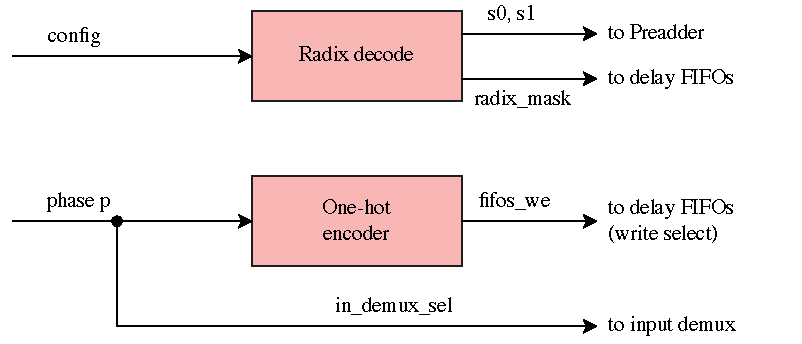
\includegraphics[width=0.9\textwidth]{figs/stage_control.pdf}
    \caption{Stage control logic.}
    \label{fig:stage_control}
\end{figure}

The radix decode block translates the configured radix into the preadder select signals \texttt{s0} and \texttt{s1} (with the values given in the preadder figures) and into \texttt{radix\_mask}, which marks the delay FIFOs used by the selected radix; the FIFOs outside the mask are held inactive. The decode is registered, which is allowed because the configuration only changes between frames; the extra cycle of latency is absorbed by the commit sequence described in the top-level control.

The input phase $p$ directly drives the select of the input demultiplexer, and the one-hot encoder turns it into the write enables of the delay FIFOs, so every incoming sample is written into the FIFO of its arm. The write enables are qualified by the stage with the input handshake, so no gating is needed inside the control logic.

\subsection{Flow Control}
\label{sec:flow_control}

The stages of the chain are connected with a ready/valid handshake on both faces. Figure \ref{fig:stage_flow_control} shows the data and control flow of one stage: the datapath in the top row and the control that steers it below, with the dashed line marking the border between the input flow and the output flow.

\begin{figure}[H]
    \centering
    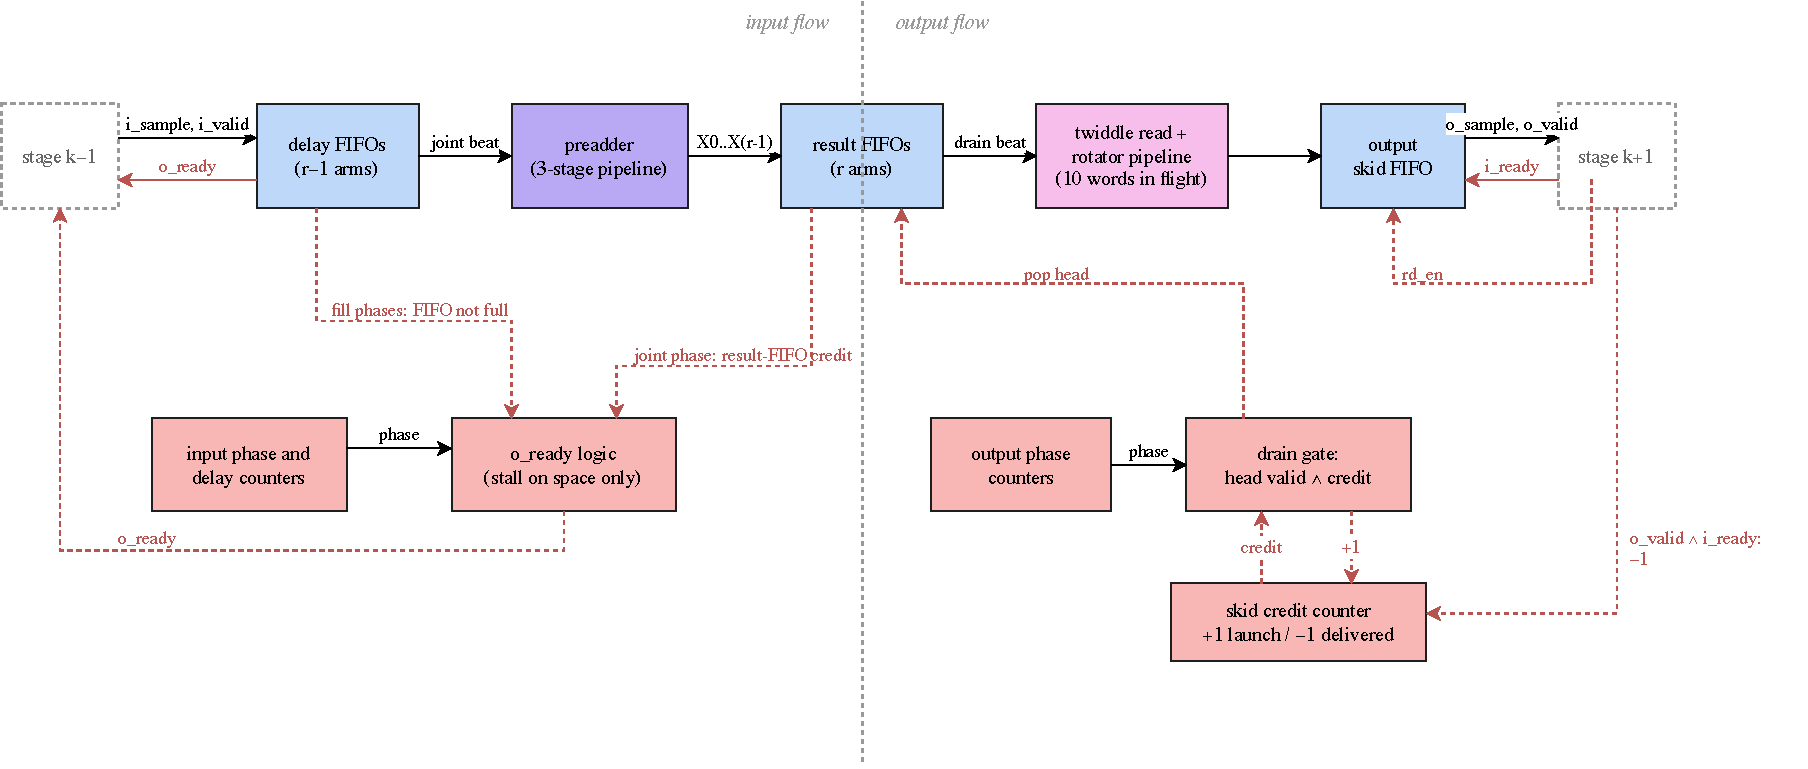
\includegraphics[width=1.0\textwidth]{figs/stage_flow_control.pdf}
    \caption{Data and control flow of the stage.}
    \label{fig:stage_flow_control}
\end{figure}

The two flows are fully decoupled and meet only in the FIFOs. The input side runs on its own phase and delay counters, and its \texttt{o\_ready} logic stalls only on space: during the fill phases on the full flags of the delay FIFOs, and during the joint phase on the credit of the result FIFOs. The downstream \texttt{i\_ready} never enters this logic and therefore cannot stall the input side directly; the stage keeps accepting samples and prefills the delay FIFOs for the next block while the results of the previous block are still being read out of the result FIFOs -- or are still waiting there because the receiving side is not ready yet.

The output side drains the result FIFOs on its own counters. A drain gate releases a result only when its FIFO head is valid and the skid credit counter shows room, because a released word then spends ten cycles in the twiddle read and the rotator pipeline and cannot be stopped anymore. If \texttt{i\_ready} drops in the meantime, the word still lands safely in the output skid FIFO, whose depth covers all words in flight plus margin. The credit counter is incremented on every drain beat and decremented on every word delivered downstream (\texttt{o\_valid} and \texttt{i\_ready}), so the skid can never overflow.

With this partitioning there is no combinational path from \texttt{i\_ready} to \texttt{o\_ready} or from \texttt{i\_valid} to \texttt{o\_valid}: \texttt{i\_ready} only pops the skid FIFO, and \texttt{o\_ready} is derived from registered FIFO state. The stages therefore chain without timing loops, and a stall on any face is absorbed locally by the FIFOs instead of rippling through the whole chain within one cycle.

\subsection{Top-level control}

The chain of stages needs top-level control logic to coordinate the reconfiguration of the stages and the data flow between the stages. It is shown in Figure~\ref{fig:top_level_control}.

\begin{figure}[p]
    \centering
    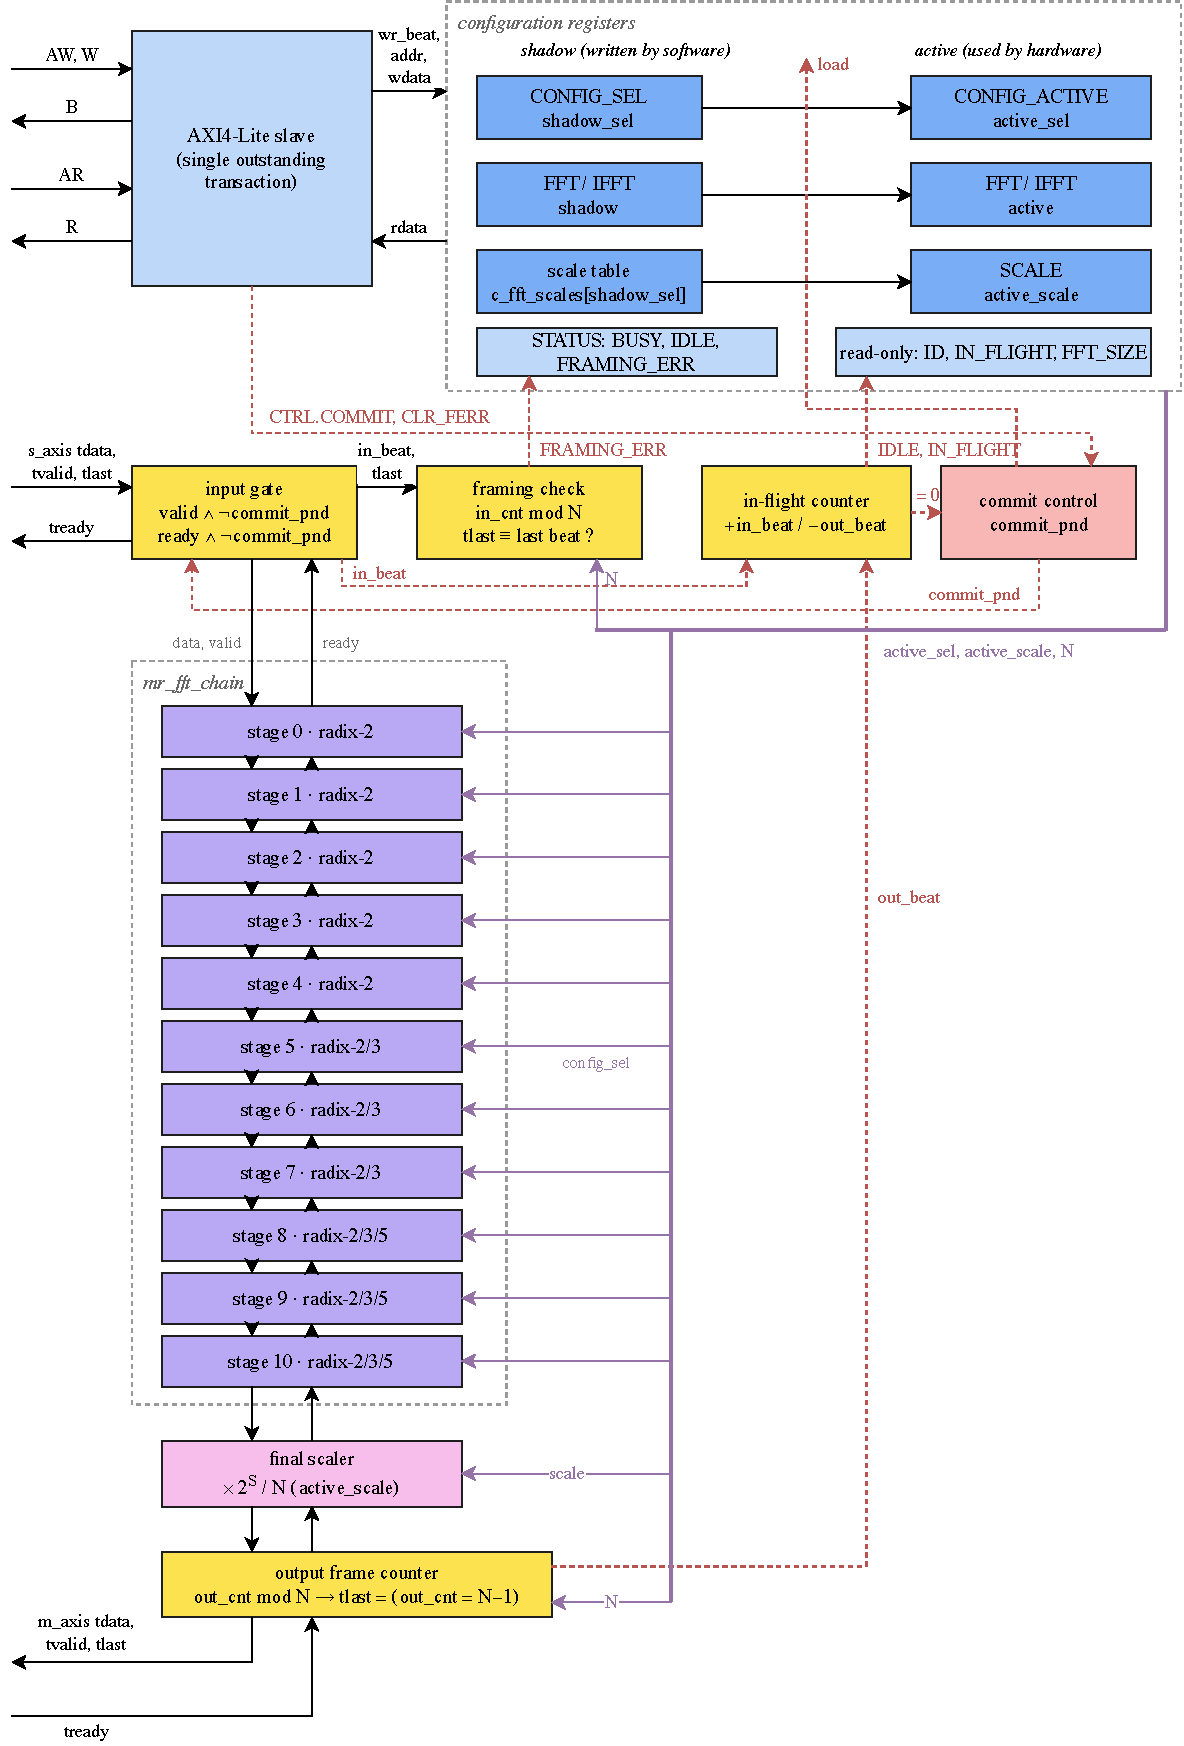
\includegraphics[width=1.0\textwidth,height=0.92\textheight,keepaspectratio]{figs/top_level_control.pdf}
    \caption{Top level: AXI4-Lite configuration interface, shadow and active registers, chain of stages and AXI4-Stream ports.}
    \label{fig:top_level_control}
\end{figure}

The core is configured over an AXI4-Lite slave with a small register map. The slave accepts the write address and data channels in the same beat and keeps a single transaction outstanding, which is sufficient for a quasi-static configuration that is written a few times per second at most. Every configurable value exists twice: software writes the shadow registers (\texttt{CONFIG\_SEL}, the FFT/IFFT flag and, derived from \texttt{CONFIG\_SEL}, the scaler constant), while the hardware only ever sees the active registers. The two are separated so that a new configuration can be written at any time without disturbing the frame that is currently in the chain.

The transfer from shadow to active is done by the commit control. A write of \texttt{CTRL.COMMIT} sets \texttt{commit\_pnd}, which closes the input gate: the input \texttt{tvalid} is masked and \texttt{tready} is held low, so no new samples enter. The in-flight counter, incremented on every accepted input beat and decremented on every delivered output beat, tells when the chain is empty; at that moment the active registers are loaded from the shadow registers in one cycle and the gate reopens. Because the stages carry no state between frames once drained, no reset is needed. \texttt{STATUS} exposes \texttt{BUSY} (commit pending) and \texttt{IDLE} (in-flight counter at zero) so the software can poll the switch, or simply keep streaming while the gate handles the boundary.

The stages inside the chain are connected only through their ready/valid handshakes, and the active configuration select is distributed to all of them. A stage whose slot is not needed by the active size bypasses itself through its output skid, so the stream is re-registered in every slot and there are no chain-level multiplexers. A bypassed slot therefore still costs one cycle of latency and one skid FIFO of storage, but in return the timing of the chain does not depend on the configuration. The final scaler multiplies the chain output by the residual gain $2^{S}/N$ of the active size (Section \ref{sec:scaling}), so that the output is delivered in the $X/N$ convention.

The AXI4-Stream \texttt{tlast} marker is not carried through the chain. The delay FIFOs are set up for the active $N$, so an input \texttt{tlast} could not steer the datapath anyway; it is only checked by the input frame counter, and a \texttt{tlast} that does not fall on the last beat of a frame sets the sticky \texttt{FRAMING\_ERR} bit in \texttt{STATUS}. On the output side \texttt{tlast} is regenerated from the output frame counter, which counts modulo the active $N$. This is exact because a commit only lands when the chain is drained, i.e. on a frame boundary, and both counters are cleared at that point.

\chapter{Software Reference Model}
\label{ch:software_model}
To implement the mixed-radix FFT algorithm in hardware, a software reference model must be developed. It is a software implementation of the mixed-radix FFT algorithm that is used for multiple purposes:
\begin{itemize}
    \item Debugging of the hardware implementation,
    \item Verification of the hardware implementation,
    \item Model performance evaluation and optimization,
    \item Fast model design iterations.
\end{itemize}

The model is implemented in the Python programming language for its simplicity, readability and ease of modification. It models all blocks of the mixed-radix FFT architecture described in this thesis -- both the control and the data path. Samples are represented as complex numbers in fixed-point format.

\section{Structure of the Model}

Two models of the chain exist side by side. The floating-point model is a direct translation of the SDF architecture into Python classes and was written first; it was used to get the control -- the phase and delay counters, the FIFO write-back and the twiddle exponent -- right before any word width was chosen. The fixed-point model has the same structure, class for class, and adds a quantizer at every place where the hardware rounds. Once the fixed-point model matched the floating-point one to within the expected rounding noise, it became the golden reference for the RTL, and every RTL block is verified against it bit for bit.

The classes of the fixed-point model mirror the RTL entities: a preadder with a capability parameter that instantiates only the ports and the constant multipliers of the selected radix set, exactly like the VHDL if-generate does; a twiddle unit that stores one octant of the unit circle and reconstructs the rest with conjugation and swaps, so that it reads the same ROM contents as the hardware; a rotator; the phase and delay counters; a delay FIFO, which is a plain list used as a shift register; the stage that connects them; and the final scaler. A chain is a list of stages built from the ascending radix factorization of $N$ with progressively divided sub-sizes -- the same placement that the VHDL elaboration functions perform for the slots -- and bypassed slots are left out, since they do not change the data.

The model is sample-accurate, not cycle-accurate. One call of a stage consumes one input sample and produces one output sample; pipeline registers, the ready/valid handshake and stalls are not modeled, so the model tells what a stage computes, and the RTL testbench takes care of when. This keeps the model short and fast enough to run the whole sweep of transform sizes, while the timing is verified in simulation by comparing the RTL output stream, after latency alignment, with the model output stream.

Fixed-point arithmetic is done with a small quantizer class of its own. A format is given by the total word width and the number of fraction bits -- 18 and 16, respectively, for the s2.16 data word -- together with a rounding mode -- truncation, round-to-nearest-even or half-up -- and an overflow mode, wrap or saturate. The quantizer maps a value onto the integer code grid of the format, rounds and wraps there, and returns the value as a double. All values that occur in the datapath are exact in a double, so no error is added by the representation itself, and the model runs about two orders of magnitude faster than with a general fixed-point library; the fxpmath library \cite{fxpmath} is kept as a reference path and the two are checked against each other. The rounding and overflow modes are parameters, so the same model was used to compare truncation with the two round-to-nearest variants; half-up was selected because it differs from round-to-nearest-even only on exact ties, which are rare in the datapath, and because it costs only a carry-in on the DSP post-adder, whereas ties-to-even needs a comparator on every rounding.

The model also generates the stimuli and expected responses for the self-checking VHDL testbenches. Separate scripts emit the vectors for the preadder in every radix mode and capability, for the twiddle ROM for every configuration and exponent, for a single stage with on-the-fly reconfiguration between delays, and for the whole chain including the final scaler. The vectors are written as integer codes, so the testbench compares words, not values, and any mismatch of a single LSB fails the test. The same model, reduced to one file, runs on the target board next to the FPGA and compares the samples returned by the core over AXI DMA with its own prediction.

\section{Fixed-Point Formats}

The word widths of the design were not fixed in advance; the model is parameterized in the width of the data word, of the preadder coefficients, of the twiddle factors and of the internal preadder words, and the signal-to-quantization-noise ratio (SQNR) was measured for the candidate widths before the RTL was written. The formats that came out of this are the ones declared in the RTL package and are listed in Table \ref{tab:fxp_formats}. The notation s$a$.$b$ stands for a signed two's-complement word with $a$ integer bits, the sign bit included, and $b$ fraction bits.

\begin{table}[H]
\centering
\caption{Fixed-point formats of the design.}
\medskip
\label{tab:fxp_formats}
\begin{tabular}{l c c l}
\hline
word & format & bits & use \\
\hline
\hline
data & s2.16 & 18 & FIFOs, links between stages, DSP B port \\
coefficient & s2.16 & 18 & preadder constants $k_2 \ldots k_6$ \\
twiddle factor & s2.16 & 18 & twiddle ROM, rotator DSP input \\
wide & s5.18 & 23 & preadder adder tree, DSP A port \\
product & s6.22 & 28 & trimmed coefficient products, their sums \\
scaler constant & s4.21 & 25 & final scaler, DSP A port \\
\hline
\end{tabular}
\end{table}

The data word is the one that matters most, because every FIFO, every link between the stages and every multiplier input carries it. Two resources of the FPGA set its size. The block RAM of the 7-series fabric of the Zynq-7000 is a 36~Kb block organized as 1024 words of 36 bits \cite{ug473}, so a complex sample with 18 bits per component fills one memory word exactly: a delay FIFO of depth up to 1024 costs one block RAM, and not a single bit of it is wasted. The multiplier of the DSP48E1 slice is asymmetric, $25 \times 18$ bits \cite{ug479}, so 18 bits is also the widest data word that fits the B port of the multiplier. Every bit taken from the word costs about $6$~dB of SQNR, and every bit added above 18 would double the memory and the DSP blocks, because neither the block RAM word nor the multiplier port can grow by one bit; therefore the s2.16 word was chosen for the data, the coefficients and the twiddle factors alike, and the SQNR in Section \ref{sec:sqnr} is what this word delivers.

Two integer bits are needed rather than one. The scaling in the preadder covers the growth of the butterflies and a rotation preserves the magnitude of a sample, so the magnitude never grows along the chain; a rotation does, however, redistribute it between the two components. An input sample with both components at full scale has a magnitude of $\sqrt{2}$, and after a rotation by $45^\circ$ one component alone carries it. The second integer bit provides this headroom, so the input may use the full $\pm 1$ range per component. The coefficient word needs the same headroom for a different reason, since $k_5 \approx 1.54$ exceeds one.

Inside the preadder, the data is wider. The adder tree of the radix-5 butterfly sums up to five inputs of magnitude up to two, so its nodes stay below sixteen in magnitude and five integer bits are enough; the algorithmic $1/2$ and $1/4$ shifts of the radix-3 and radix-5 butterflies need two more fraction bits to remain exact. The resulting s5.18 word has 23 bits and rides on the 25-bit A port of the DSP48E1, so the whole multiplier is used and the adder tree is computed without any rounding. The product of the 23-bit wide word and the 18-bit coefficient is 41 bits long; it is trimmed once to 22 fraction bits with half-up rounding, the rounding constant being added on the post-adder of the DSP slice, and the sums of the trimmed products fit in six integer bits. This s6.22 product word is what enters the $\gg s$ rnd blocks of the preadder, where it is scaled and rounded back to s2.16 in one step, as described in Section \ref{sec:scaling}. In this way the preadder rounds each output exactly once, no matter how many adder levels it passes.

The final scaler multiplies the s2.16 data on the B port by a constant on the A port. The constant $2^{S}/N$ lies between $4/3$ and about $5.7$, so it needs four integer bits, and 21 fraction bits keep its relative error near $-135$~dB, far below the rounding noise of the chain, at no extra cost since the port is 25 bits wide anyway.

\section{SQNR Evaluation}
\label{sec:sqnr}

The SQNR of the fixed-point chain was measured against a double-precision FFT for all 53 supported sizes. The stimulus is a frame of $N$ samples of complex white Gaussian noise, the classical input for the noise analysis of fixed-point FFTs \cite{oppenheim_weinstein}: the samples are independent, so the rounding errors of all butterflies are uncorrelated and the measured SQNR is the average behavior of the datapath rather than the response to one particular signal. The real and imaginary parts are drawn independently with a standard deviation of $\sigma = 0.225$, so that the $4\sigma$ peaks reach $0.9$ of full scale ($-1$~dBFS), the input level the chain is specified for; the rare samples beyond $\pm 4\sigma$ are clipped to $\pm 0.9$ rather than allowed to wrap in the s2.16 input word. The model chain is built for $N$ exactly as the hardware would be configured -- ascending radices, s2.16 words, half-up rounding, the fixed scaling schedule, exit rounding with 22-bit products and the quantized final scaler -- and the frame is streamed through it followed by a zero frame that flushes the pipeline. The output stream is taken from the chain latency onward, reordered from digit-reversed to natural order and compared with $X_k = \mathrm{FFT}(x)/N$ computed by NumPy in double precision. With the error $e_k = X_k - \hat{X}_k$ the SQNR is

\begin{equation}
    \mathrm{SQNR} = 10 \log_{10} \frac{\sum_{k} |X_k|^2}{\sum_{k} |e_k|^2},
\end{equation}

where both sums run over all bins of all frames. Sixty-four frames with different random seeds are used per size, and the signal and error powers are accumulated over the frames before the ratio is formed, so the result is a proper power average and not a mean of decibel values; with this many frames the statistical scatter between runs is well below $0.1$~dB, and every feature left in the curve is a property of the datapath. The result for every supported size is shown in Figure \ref{fig:sqnr_noise}.

\begin{figure}[H]
    \centering
    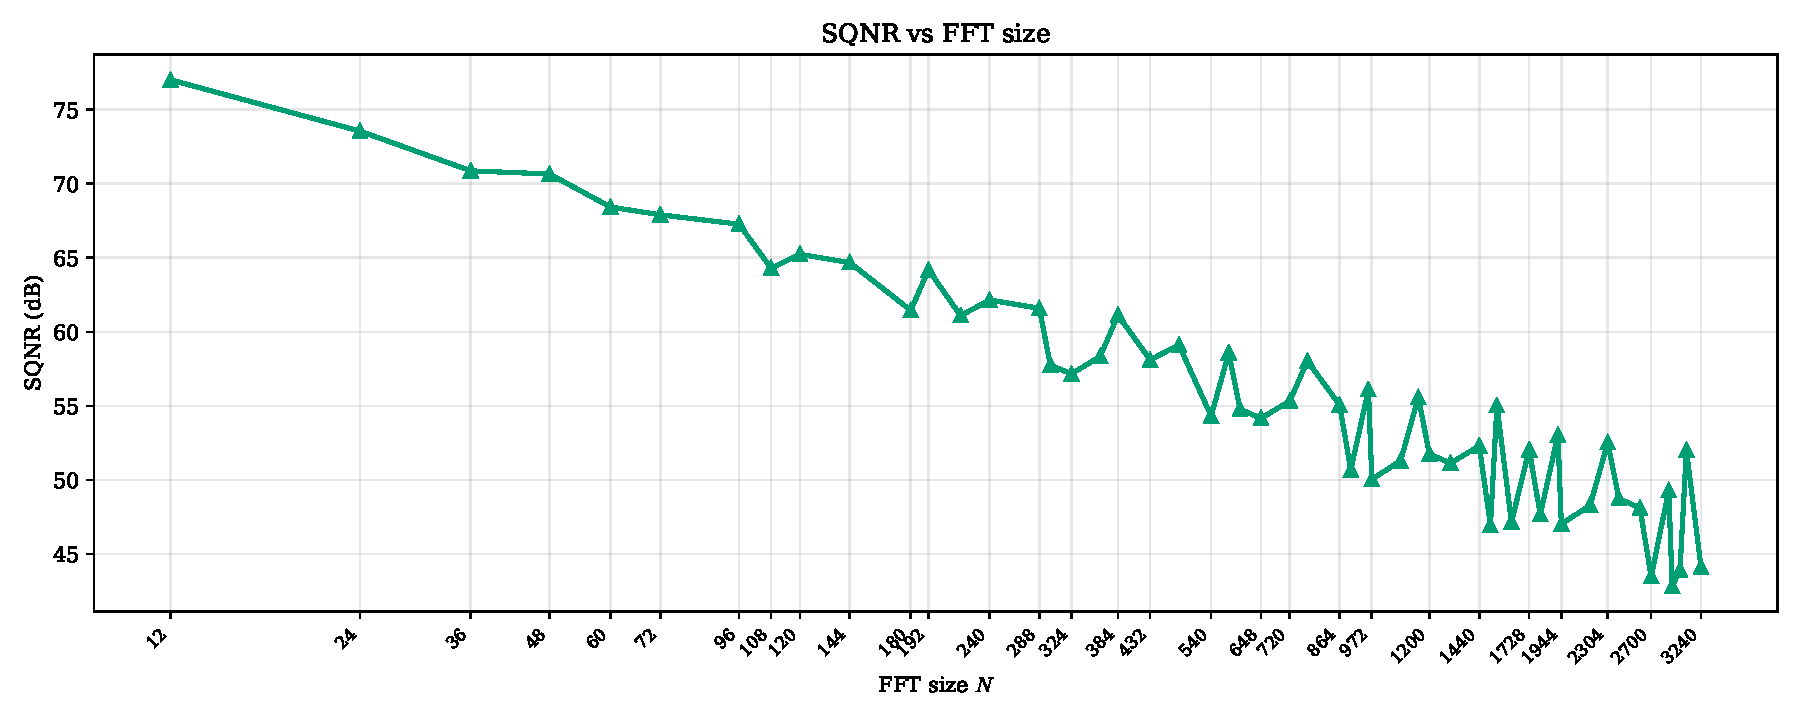
\includegraphics[width=1.0\textwidth]{figs/sqnr_rounding_sweep.pdf}
    \caption{SQNR of the fixed-point chain for complex white Gaussian noise input at $-1$~dBFS peak, 64 frames per point, all 53 supported sizes.}
    \label{fig:sqnr_noise}
\end{figure}

The SQNR falls from $77$~dB at $N = 12$ to $43$~dB at $N = 2916$, by about $4$~dB per doubling of $N$ on average, as expected: every additional stage adds its own rounding noise while the fixed scaling keeps the signal level constant, so the noise power grows roughly in proportion to $N$. Two effects are visible on top of this trend. Sizes with many radix-3 and radix-5 stages sit below their neighbors -- $N = 2916 = 4 \cdot 3^6$ reaches $43$~dB, whereas $N = 3072 = 2^{10} \cdot 3$ reaches $52$~dB -- because a radix-3 or radix-5 stage divides by four or eight instead of by three or five, so the signal loses $2.5$ or $4.1$~dB of level in every such stage and the final scaler amplifies the rounding noise of all later stages by the same amount.

A coherent tone at a bin center can be used as a second stimulus; it does not measure the average noise -- for a coherent tone the chain concentrates practically its whole rounding error into the fundamental bin, at most about one LSB, and leaves every other bin exact -- but it confirms that the datapath produces no spurious components above the quantization floor. The three rounding modes of the quantizer can be swept in one run with any of these stimuli, which is how half-up rounding was selected.

\chapter{Results}
\label{ch:results}

\section{Implementation and Verification Flow}

The design is written in VHDL-2008. All parameters of the chain -- the number of slots, the capability of every slot, the configuration table of every stage, the FIFO depths, the twiddle tables and the scaler constants -- are computed at elaboration time from two constants, the base size $12$ and the upper limit $3300$, by the functions of the package described in the previous chapters, so nothing in the RTL is written by hand for a particular set of FFT sizes.

Simulation was done with GHDL \cite{ghdl}. The XSim simulator of Vivado cannot handle a design of this size: its debug database breaks on the very large elaboration-time constants of the configuration package, whereas GHDL analyzes and simulates the whole chain with all 53 configurations without difficulty. The verification is organized bottom-up with self-checking testbenches for the FIFO, the preadder in every capability and radix mode, the twiddle ROM for every configuration and exponent, a single stage of every capability with reconfiguration on the fly between delays, and the complete top level with the chain and the final scaler. All expected responses are produced by the Python model of Chapter \ref{ch:software_model} and written as integer codes; a testbench compares words, so the RTL is proven bit-exact against the model, and the SQNR figures measured on the model in Section \ref{sec:sqnr} therefore apply to the hardware as well.

Synthesis and implementation were done with Vivado 2022.2, because this is the version that the PYNQ v3.0.1 image of the target board is built with \cite{pynq}, so the generated bitstream and hardware description can be loaded by the PYNQ overlay class directly. The target is the PYNQ-Z2 board shown in Figure \ref{fig:pynq_z2}, with a Zynq-7000 XC7Z020-1CLG400 SoC \cite{ug585}, whose programmable logic is an Artix-7 fabric with 53200 LUTs, 106400 flip-flops, 140 block RAM tiles of 36~Kb and 220 DSP48E1 slices. The board is driven over Ethernet from a host computer; the Zynq processing system runs the PYNQ Linux image with a Jupyter server, and the test scripts of the model run on the ARM cores and talk to the FFT core through the AXI DMA and the AXI4-Lite register interface.

\begin{figure}[H]
    \centering
    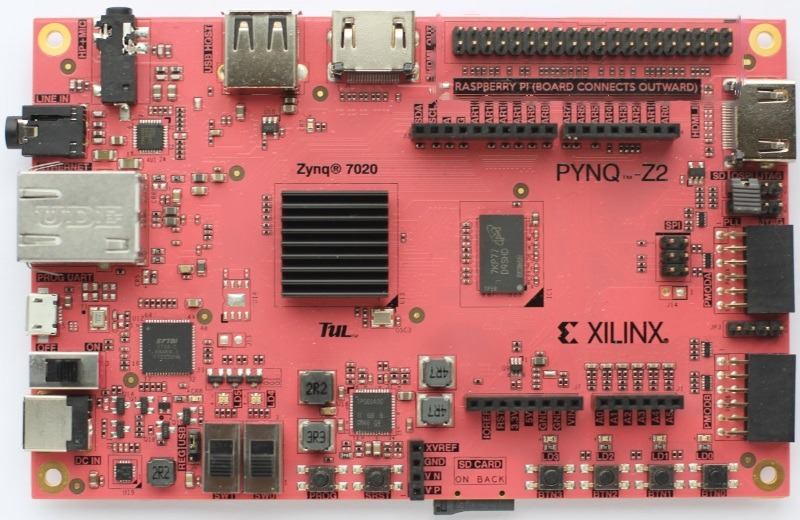
\includegraphics[width=0.8\textwidth]{figs/pynq_z2.jpg}
    \caption{PYNQ-Z2 development board with the Zynq-7000 XC7Z020 SoC \cite{pynq}.}
    \label{fig:pynq_z2}
\end{figure}

\section{Block Design}

The FFT core is packaged as an IP and connected to the processing system as shown in Figure \ref{fig:block_design}. The processing system exposes one general-purpose AXI master port and one high-performance AXI slave port. The general-purpose port reaches, through an AXI interconnect, the AXI4-Lite slave of the FFT core and the register interface of an AXI DMA; the software configures the core and programs the DMA through this path. The DMA has a memory-mapped side connected through a second interconnect to the high-performance port, from where it reads and writes the DDR memory of the board, and a streaming side with a 64-bit AXI4-Stream master and slave that are connected to the input and the output of the FFT core. A processor system reset block distributes the reset, and the single clock of the design is the fabric clock of the processing system.

\begin{figure}[H]
    \centering
    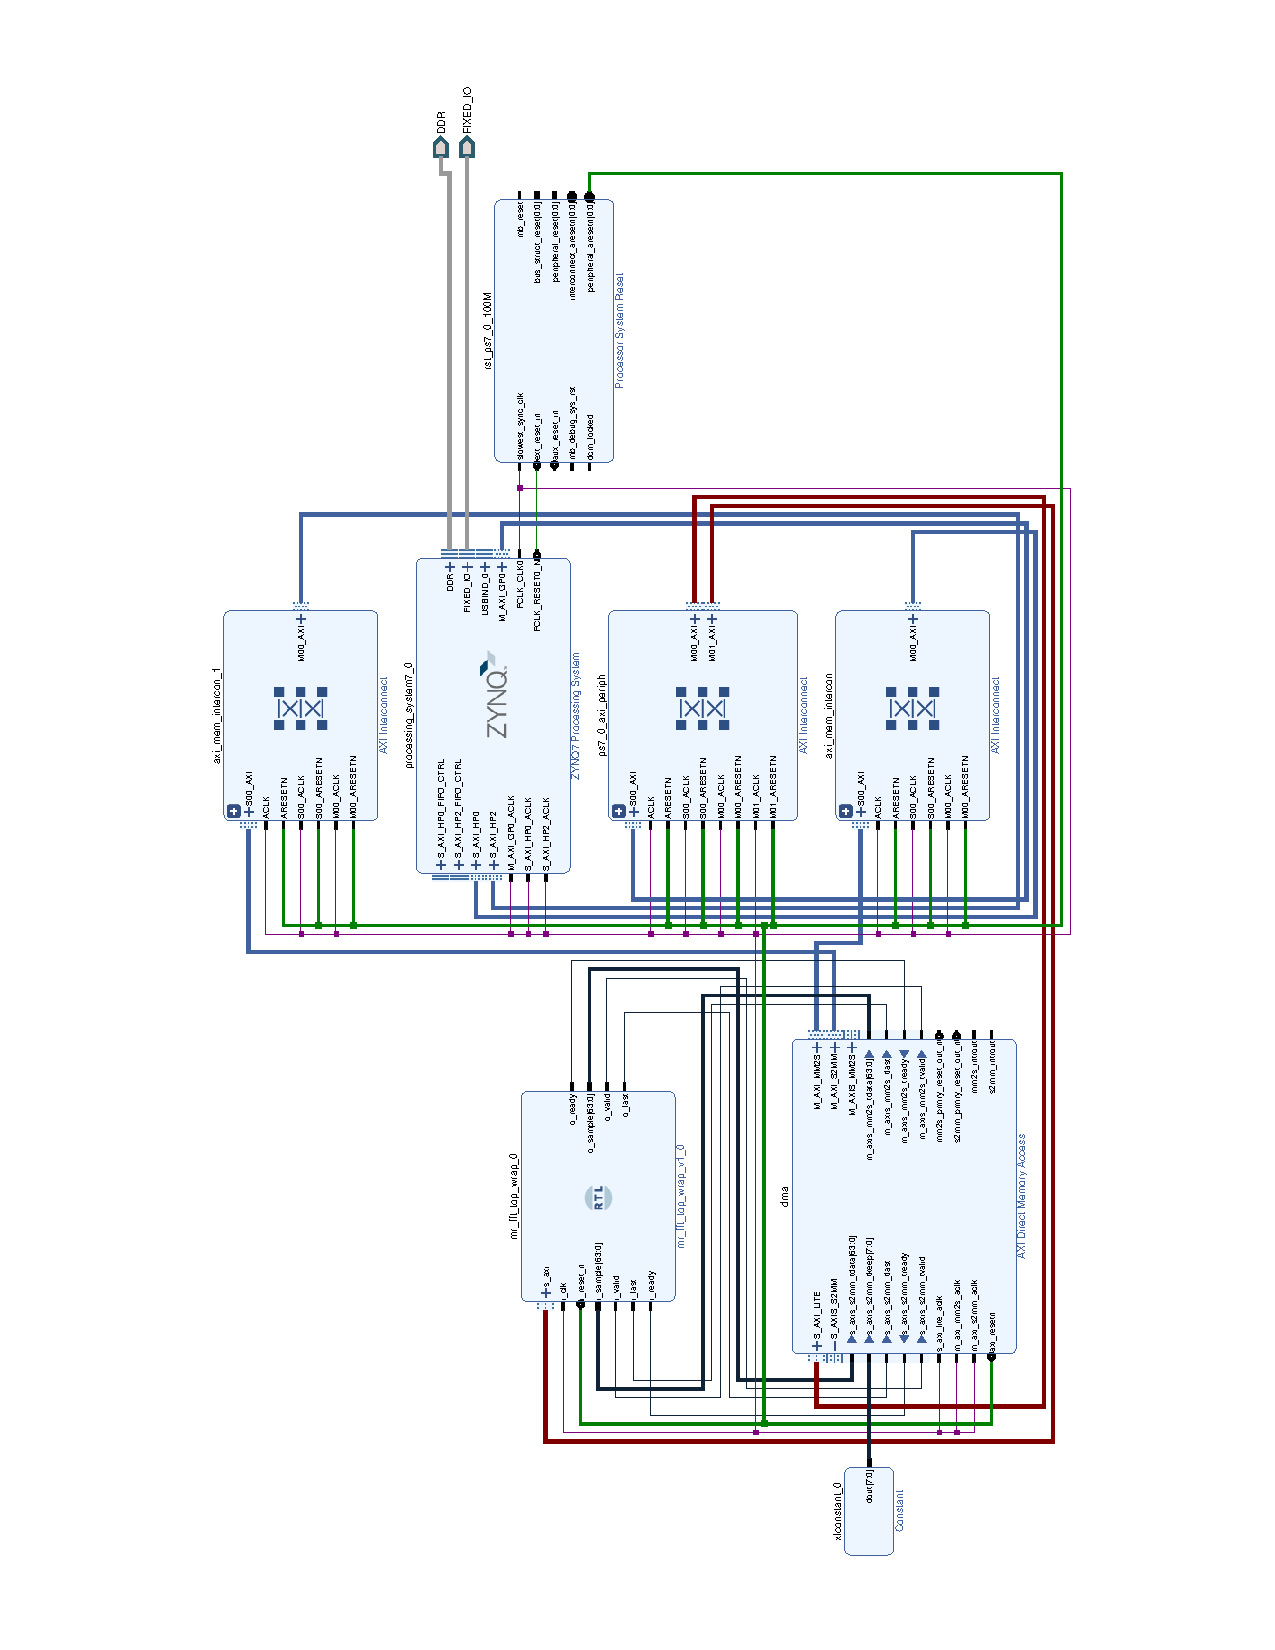
\includegraphics[trim=101 45 98 41,clip,angle=-90,width=1.0\textwidth]{figs/my_block_diagram.pdf}
    \caption{Vivado block design: processing system, AXI DMA, AXI interconnects and the FFT IP.}
    \label{fig:block_design}
\end{figure}

One 64-bit stream beat carries one complex sample: the real part in bits 17 to 0 and the imaginary part in bits 35 to 18, both as s2.16 codes, with the upper bits unused. A transform is run from a Jupyter notebook on the ARM cores in a few lines: the \texttt{CONFIG\_SEL} register is written with the index of the desired size, \texttt{CTRL.COMMIT} is written, \texttt{STATUS} is polled until the switch is done, and then one DMA transfer of $N$ beats is started in each direction. The chain delivers its output in digit-reversed order, and the software applies the permutation for the configured $N$ before comparing with a NumPy reference; nothing else is needed, since the final scaler already delivers the $X_k/N$ convention.

\section{Order of Stages and Memory Budget}
\label{sec:memory_budget}

The slots of the chain are ordered radix-2 first, then radix-2/3, then radix-2/3/5. The reason is memory. The storage of an SDF chain is concentrated in its first stages, since the delay of a stage is $N/r$ and shrinks by the radix from stage to stage; the first stage alone holds close to half of all samples in flight. A radix-2 stage has one delay FIFO and nothing else, whereas a radix-2/3 stage has two delay FIFOs and two result FIFOs and a radix-2/3/5 stage four of each. Placing the stages with the most buffers where the buffers are deepest would multiply the largest depth by eight; placing them at the end, where the depth is a few dozen words, makes the eight buffers nearly free. The radix-2 slots, which need a single deep FIFO each, are therefore put at the head of the chain, where their depth of up to 1620 words maps onto one or two block RAMs with the 36-bit word fully used.

Table \ref{tab:slot_memory} lists the buffers of every slot as they are elaborated from the set of supported sizes. The delay FIFO depth is the largest $N/r$ that any configuration assigns to the slot, the result FIFO depth adds the preadder latency and a margin of two words, and the output skid FIFO has a fixed depth of 15 words, or 14 in the radix-2/3/5 slots, whose twiddle ROM is read one cycle faster from the fabric. The twiddle ROMs themselves are not counted here. The last column counts 36~Kb block RAMs: a FIFO of depth up to 512 fits half a block, up to 1024 a whole block, and deeper FIFOs are cascaded; FIFOs below 128 words are mapped onto distributed RAM in the fabric and take no block RAM at all.

\begin{table}[H]
\centering
\caption{Buffer storage of the eleven slots, in words of 36 bits.}
\medskip
\label{tab:slot_memory}
\setlength{\tabcolsep}{4.5pt}
\begin{tabular}{c l c c c r c}
\hline
slot & capability & delay FIFOs & result FIFOs & skid & words & BRAM \\
\hline
\hline
0  & radix-2     & $1 \times 1620$ & --             & 15 & 1635 & 2   \\
1  & radix-2     & $1 \times 810$  & --             & 15 & 825  & 1   \\
2  & radix-2     & $1 \times 405$  & --             & 15 & 420  & 0.5 \\
3  & radix-2     & $1 \times 192$  & --             & 15 & 207  & 0.5 \\
4  & radix-2     & $1 \times 96$   & --             & 15 & 111  & --  \\
5  & radix-2/3   & $2 \times 243$  & $2 \times 248$ & 15 & 997  & 2   \\
6  & radix-2/3   & $2 \times 81$   & $2 \times 86$  & 15 & 349  & --  \\
7  & radix-2/3   & $2 \times 27$   & $2 \times 32$  & 15 & 133  & --  \\
8  & radix-2/3/5 & $4 \times 25$   & $4 \times 30$  & 14 & 234  & --  \\
9  & radix-2/3/5 & $4 \times 5$    & $4 \times 10$  & 14 & 74   & --  \\
10 & radix-2/3/5 & $4 \times 1$    & $4 \times 6$   & 14 & 42   & --  \\
\hline
\multicolumn{5}{r}{total} & 5027 & 6 \\
\hline
\end{tabular}
\end{table}

The whole chain buffers about 5000 words and its FIFOs take six block RAMs, with the two radix-2 slots at the head and the first radix-2/3 slot accounting for five of them. For comparison, the same set of sizes placed in the reverse order -- radix-2/3/5 slots first, so that the radix-5 and radix-3 factors are taken out of $N$ first -- was evaluated with the same elaboration rules: the first slot alone would then need four delay FIFOs of 1024 words and four result FIFOs of 1029 words, the chain would buffer about 15500 words and take 24 block RAMs, three times the storage and four times the block RAM of the chosen order. The order of the radices does not change the transform, only the digit-reversal permutation at the output, so the memory alone decides it.

\section{Resource Utilization}
\label{sec:utilization}

Table \ref{tab:utilization} lists the utilization of the placed design as reported by Vivado. The core takes about a third of the LUTs and DSP slices and a quarter of the block RAM of the device, and 12\% of the flip-flops.

\begin{table}[H]
\centering
\caption{Utilization of the placed design on the XC7Z020.}
\medskip
\label{tab:utilization}
\begin{tabular}{l r r r}
\hline
resource & used & available & utilization \\
\hline
\hline
Slice LUTs & 17538 & 53200 & 33.0\% \\
\quad LUT as logic & 15774 & 53200 & 29.7\% \\
\quad LUT as distributed RAM & 1536 & 17400 & 8.8\% \\
\quad LUT as shift register & 228 & 17400 & 1.3\% \\
Slice registers & 12780 & 106400 & 12.0\% \\
Slices & 5681 & 13300 & 42.7\% \\
Block RAM tiles (36~Kb) & 34 & 140 & 24.3\% \\
\quad RAMB36 & 29 & 140 & 20.7\% \\
\quad RAMB18 & 10 & 280 & 3.6\% \\
DSP48E1 & 72 & 220 & 32.7\% \\
\hline
\end{tabular}
\end{table}

The 72 DSP slices are accounted for exactly by the arithmetic described in Chapter \ref{ch:hardware_architecture}. Ten of the eleven slots have a rotator with four multipliers each, 40 slices; the last slot has a delay of one and rotates only by $W^0 = 1$, so its rotator degenerates to a register and takes none. The three radix-2/3/5 preadders take eight slices each for the shared $k_6/k_2$ multiplier and the three purely imaginary coefficients, the three radix-2/3 preadders two slices each for $k_6$, and the final scaler two -- $40 + 24 + 6 + 2 = 72$. No multiplier is built in the fabric, and the half-up rounding constants and the pipeline registers of the multipliers are absorbed into the slices, as intended.

The block RAM tiles are more than the six blocks estimated for the FIFOs in Section \ref{sec:memory_budget}. On top of the FIFOs, the twiddle ROMs add a large amount of storage: every radix-2 and radix-2/3 slot holds the octant tables of all of its configurations in one block ROM, and the first slot alone stores about 7200 words of 36 bits for its 53 configurations. The eight block-ROM slots together account for about 22 blocks, and the rest of the 34 tiles is the granularity of the mapping onto RAMB36 and RAMB18 primitives. The 1536 LUTs used as distributed RAM are the small FIFOs of the later slots, below 128 words, and the twiddle tables of the radix-2/3/5 slots. The twiddle storage is thus the larger part of the memory of the design, and it can be reduced considerably, as described in the next chapter.

\section{Timing}

The design meets a clock period of $7.6$~ns after routing, with a worst negative slack of $+0.043$~ns and no failing endpoints. The maximum clock frequency is therefore $131.6$~MHz, and since the chain processes one sample per clock cycle in every configuration, this is also the throughput in samples per second.

\section{Measurements on the Board}

The same test that was run on the top level in simulation was repeated on the PYNQ-Z2 board over the DMA path of Figure \ref{fig:block_design}: the input frames of the chain testbench were streamed through the core for every supported size, the output was read back, reordered from digit-reversed to natural order and compared word by word with the output of the Python model. The core output was bit-exact with the model in every configuration, so the SQNR figures of Section \ref{sec:sqnr} are the ones the hardware delivers.

\chapter{Future Work}
\label{chap:future_work}

The design has several potential areas for improvement, and this chapter discusses some of them.

\section{Reduction of Twiddle Storage}
\label{sec:twiddle_reduction}

The twiddle tables are the largest part of the memory of the design, an observation also made in \cite{yang2023}, where the sharing and compression of the twiddle factors between the modes is one of the main measures of the architecture. In the current implementation every slot stores one octant table for every one of its configurations, so the first slot alone holds 53 tables with about 7200 words, and the whole chain about 18500 words. Most of this storage is redundant: the twiddle factors of an FFT of size $N$ are a subset of the twiddle factors of every size $M$ that is a multiple of $N$, since
\begin{equation}
    W_N^{k} = e^{-j \frac{2\pi k}{N}} = e^{-j \frac{2\pi s k}{M}} = W_M^{sk}, \qquad s = \frac{M}{N}.
    \label{eq:twiddle_stride}
\end{equation}
The table of $W_M$ therefore contains the whole table of $W_N$; the entries of the smaller size are found by reading every $s$-th entry of the larger one. The stored values are also identical, since the angle $2\pi k/N$ is the same angle as $2\pi s k/M$ and the rounding to the twiddle format is done on the same real number, so the outputs of the core stay bit-exact.

The supported sizes can thus be grouped so that all sizes of one group divide the largest size of the group, and only the table of that largest size has to be stored. A size may divide several of the largest sizes, in which case it is assigned to any one of them. For the set of 53 sizes of this design there are 14 sizes that are not a divisor of any other supported size -- 1728, 1800, 1920, 1944, 2160, 2304, 2400, 2592, 2700, 2880, 2916, 3000, 3072 and 3240 -- so 14 tables cover the first slot, in place of 53. Every following slot sees the sub-FFT sizes of the previous one divided by the radix of the stage, so the same grouping repeats with smaller numbers: the second slot also needs 14 tables, the third 12, and the number falls toward the end of the chain, where the last slot needs only the tables of $W_3$ and $W_5$. Table \ref{tab:twiddle_groups} lists the number of tables and the stored words for every slot.

\begin{table}[H]
\centering
\caption{Twiddle storage per slot: separate table per configuration versus one table per divisibility group.}
\medskip
\label{tab:twiddle_groups}
\begin{tabular}{c c r r r r}
\hline
slot & capability & configurations & groups & words now & words grouped \\
\hline
\hline
0 & radix-2 & 53 & 14 & 7189 & 4345 \\
1 & radix-2 & 53 & 14 & 4372 & 2528 \\
2 & radix-2 & 39 & 12 & 1844 & 1229 \\
3 & radix-2 & 27 & 8 & 615 & 338 \\
4 & radix-2 & 19 & 7 & 277 & 176 \\
5 & radix-2/3 & 53 & 9 & 2784 & 1162 \\
6 & radix-2/3 & 39 & 6 & 799 & 323 \\
7 & radix-2/3 & 27 & 5 & 248 & 111 \\
8 & radix-2/3/5 & 38 & 4 & 322 & 87 \\
9 & radix-2/3/5 & 17 & 3 & 68 & 20 \\
10 & radix-2/3/5 & 4 & 2 & 10 & 5 \\
\hline
total & & & & 18528 & 10324 \\
\hline
\end{tabular}
\end{table}

The change to the twiddle factor unit of Figure \ref{fig:twiddle_factor_unit} is small. The configuration parameters block supplies, instead of the base address and size of the selected configuration, the base address and size $M$ of its group together with the stride $s$ of Equation \eqref{eq:twiddle_stride}. The octant fold and the reconstruct block are left as they are and work on the size $M$. The exponent accumulator, which in the current design is incremented by the arm index $p$ on every beat, is incremented by $p \cdot s$ instead; this increment is a constant of the selected configuration, so it is read from the configuration table and no multiplier is added. The exponent $sk$ stays below $M$ by construction, exactly as $k$ stays below $N$ in the current design, so the fold thresholds need no change either. The radix mode of the stage plays no part in the grouping, since a table depends only on the sub-FFT size; in the radix-2/3 and radix-2/3/5 slots the odd sizes of the radix-3 and radix-5 modes are simply grouped among themselves, as exemplified by the table of $W_{729}$ in the first radix-2/3 slot.

Grouping the tables removes about 44\% of the twiddle words, and the first slot drops from eight to five block RAMs. The remaining redundancy is between the groups: the tables of 2880 and 2160, for example, share every entry whose angle is a multiple of $2\pi/720$. Removing this as well would need a table of the least common multiple of all sizes, which is far too large, or a table of $W_M$ for a size $M$ that is not supported itself, from which every supported size is read with a rational rather than an integer stride. The latter is not possible with a plain address counter, so the grouping by divisibility is the practical limit of this approach, and further reduction would have to come from a different twiddle generation method, such as a coarse-fine decomposition of the angle with a second, small table and a complex multiplier.

\section{Digit inversion}
\label{sec:digit_inversion_unit}

The chain delivers its output in digit-reversed order, and the reordering to natural order is left to software. It can be moved into the core with the sample rearrange unit of Figure \ref{fig:sample_rearrange_unit}: two buffers of $N$ words work in ping-pong fashion, a frame is written into one buffer at the linear index $n$ while the previous frame is read out of the other at the digit-inverted index $\tilde{n}$ of Equation \eqref{eq:mixed_radix_inversion}, and the buffers swap roles when the frame counter reaches $N$. The read address is supplied by the digit inversion unit.

\begin{figure}[htb]
    \centering
    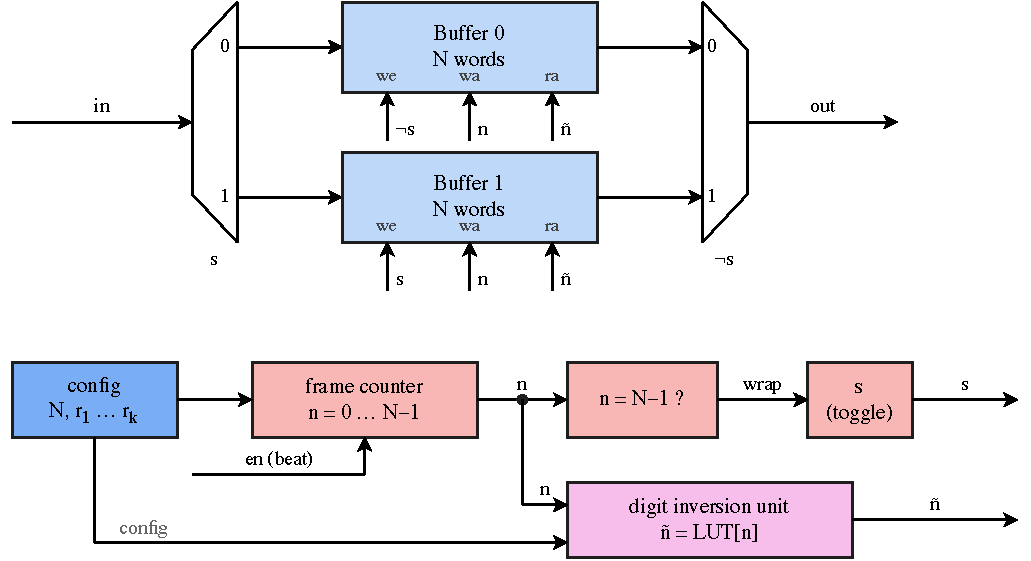
\includegraphics[width=0.9\textwidth]{figs/sample_rearrange_unit.pdf}
    \caption{Sample rearrange unit with ping-pong buffers addressed by the digit inversion unit.}
    \label{fig:sample_rearrange_unit}
\end{figure}

Forming $\tilde{n}$ for every sample would need a mixed-radix digit decomposition per beat, so the digit inversion unit of Figure \ref{fig:digit_inversion_unit} computes the permutation once after every reconfiguration and stores it in a look-up table of $N$ words that is then read at line rate. The radices of the selected size are held in the configuration registers, and a small FSM sequences the generation, as shown in Figure \ref{fig:digit_inversion_lut_gen}. The output weights calculator first forms the place values $W'_i = N/(r_k r_{k-1} \cdots r_i)$ of Equation \eqref{eq:mixed_radix_inversion} with one multiplication per radix. The digit inverter then runs through all $N$ indices with cascaded digit counters, one per radix, each wrapping at its own $r_i$ and incrementing the next, so that at every step the counters hold the digits $d_i$ of $n$; $\tilde{n}$ is accumulated as the sum of the digits weighted by $W'_i$ with one shared multiplier and adder, and written into the look-up table at address $n$. The generation runs once per configuration change, so it is absorbed into the switch time and no arithmetic sits in the sample path.
Another way to generate the digit-inverted indices would be to load them from software directly into the LUT.

The cost is the storage: the table and the two buffers add about nine block RAMs for $N = 3240$, more than all the FIFOs of the chain, which is why the reordering was left entirely to the software side in this work.

\begin{figure}[htb]
    \centering
    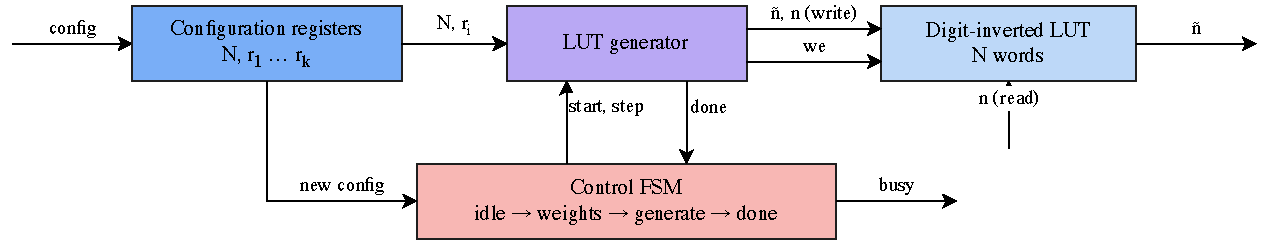
\includegraphics[width=1.0\textwidth]{figs/digit_inversion_unit.pdf}
    \caption{Digit inversion unit.}
    \label{fig:digit_inversion_unit}
\end{figure}

\begin{figure}[htb]
    \centering
    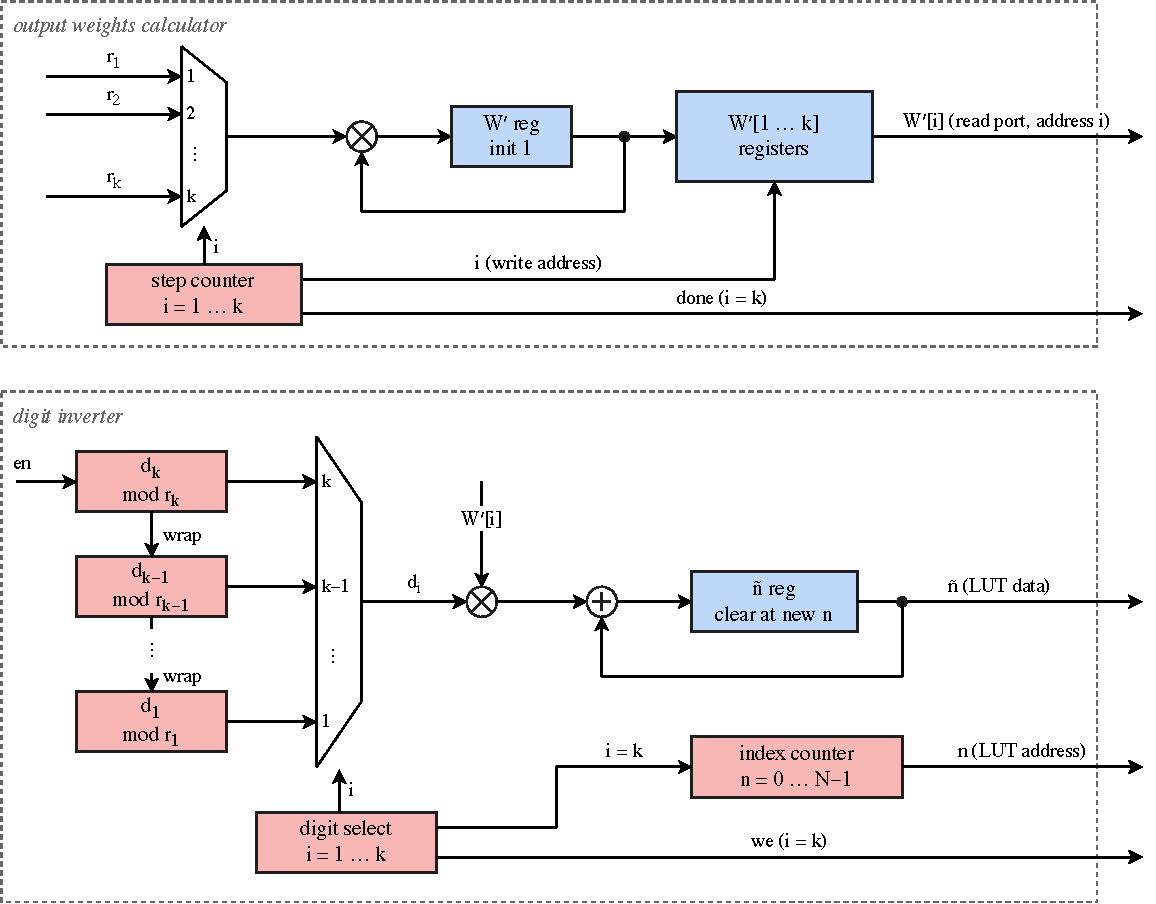
\includegraphics[width=1.0\textwidth]{figs/digit_inversion_lut_gen.pdf}
    \caption{Digit-inverted look-up table generator: output weights calculator and digit inverter.}
    \label{fig:digit_inversion_lut_gen}
\end{figure}

\chapter{Conclusion}
\label{ch:conclusion}

A run-time reconfigurable mixed-radix FFT core was designed, modeled, implemented in VHDL, and verified on an FPGA. The core supports the 53 transform sizes of the form $12 \cdot 2^i 3^j 5^k$ up to 3240 that appear in OFDM systems, and switches between them by a register write without a change of the bitstream. The single-path delay feedback architecture was extended to reconfigurable stages: eleven stages of three capabilities are connected in a chain, every stage is programmed with its radix and delay per configuration, and unused stages are bypassed, so a single datapath serves all sizes at one sample per clock cycle.

The design decisions were driven by the target technology. The reconfigurable preadders were built so that all complex coefficient products reduce to two real multiplications each, the twiddle factors are stored as octant tables in block RAM and reconstructed with multiplexers, the delay and result FIFOs are reconfigured in depth without duplicated storage, and the stages are ordered so that the deepest buffers sit in the slots with the fewest FIFOs. The scaling of the datapath was kept to a fixed shift per stage and a single final scaler, and all number formats were chosen around the 36-bit block RAM word and the $25 \times 18$ multiplier of the DSP48E1 slice.

A bit-exact Python model of the core was written and used to select these formats and to measure the quantization noise: with an s2.16 datapath the SQNR for white-noise input at $-1$~dBFS lies between $77$~dB for the smallest and $43$~dB for the largest transform. The same model produced the expected responses for the RTL testbenches, and the implemented core was proven bit-exact against it both in simulation and on the PYNQ-Z2 board over the AXI DMA path. On the XC7Z020 the core occupies 33\% of the LUTs, 33\% of the DSP slices and 24\% of the block RAM, and runs at $131.6$~MHz. The improvements identified for the design are discussed in Chapter \ref{chap:future_work}.

\thebibliography{10}

\bibitem{groginsky1970} H. Groginsky and G. Works, “A pipeline fast Fourier transform,” IEEE Transactions on Computers, vol. C-19, no. 11, pp. 1015–1019, 1970.

\bibitem{singleton1969} R. C. Singleton, “An algorithm for computing the mixed radix fast Fourier transform,” IEEE Transactions on Audio and Electroacoustics, vol. AU-17, no. 2, pp. 93–103, June 1969.

\bibitem{lofgren2011} J. Löfgren and P. Nilsson, “On hardware implementation of radix 3 and radix 5 FFT kernels for LTE systems,” in Proc. NORCHIP, Lund, Sweden, 2011, pp. 1–4.

\bibitem{qureshi2013} F. Qureshi, M. Garrido and O. Gustafsson, “Unified architecture for 2, 3, 4, 5, and 7-point DFTs based on Winograd Fourier transform algorithm,” Electronics Letters, vol. 49, no. 5, pp. 348–349, February 2013.

\bibitem{shih2018} X.-Y. Shih, H.-R. Chou and Y.-Q. Liu, “Design and implementation of flexible and reconfigurable SDF-based FFT chip architecture with changeable-radix processing elements,” IEEE Transactions on Circuits and Systems I: Regular Papers, vol. 65, no. 11, pp. 3942–3955, November 2018.

\bibitem{yang2023} C. Yang, J. Wu, S. Xiang, L. Liang and L. Geng, “A high-throughput and flexible architecture based on a reconfigurable mixed-radix FFT with twiddle factor compression and conflict-free access,” IEEE Transactions on Very Large Scale Integration (VLSI) Systems, vol. 31, no. 10, pp. 1472–1485, October 2023.

\bibitem{bautista2023} V. M. Bautista, M. Garrido and M. López-Vallejo, “Serial butterflies for non-power-of-two FFT architectures in 5G and beyond,” IEEE Transactions on Circuits and Systems I: Regular Papers, vol. 70, no. 10, pp. 3992–4003, October 2023.

\bibitem{oppenheim_weinstein} A. V. Oppenheim and C. J. Weinstein, “Effects of finite register length in digital filtering and the fast Fourier transform,” Proceedings of the IEEE, vol. 60, no. 8, pp. 957–976, 1972.

\bibitem{12} ARM, \emph{AMBA 4 AXI4-Stream protocol}, https://developer.arm.com/documentation/ihi0051/a/.

\bibitem{17} 3GPP, \emph{TS 38.211: NR; Physical channels and modulation}, V18.2.0, 3rd Generation Partnership Project, 2024.

\bibitem{18} 3GPP, \emph{TS 38.104: NR; Base Station (BS) radio transmission and reception}, V18.5.0, 3rd Generation Partnership Project, 2024.

\bibitem{ts38101} 3GPP, \emph{TS 38.101-1: NR; User Equipment (UE) radio transmission and reception; Part 1: Range 1 Standalone}, V18.5.0, 3rd Generation Partnership Project, 2024.

\bibitem{ug479} Xilinx, \emph{7 Series DSP48E1 Slice User Guide}, UG479 (v1.10), March 2018.

\bibitem{ug473} Xilinx, \emph{7 Series FPGAs Memory Resources User Guide}, UG473 (v1.14), July 2019.

\bibitem{ug585} Xilinx, \emph{Zynq-7000 SoC Technical Reference Manual}, UG585 (v1.14), June 2023.

\bibitem{pynq} AMD, \emph{PYNQ: Python productivity for Zynq}, v3.0.1, http://www.pynq.io/.

\bibitem{ghdl} T. Gingold et al., \emph{GHDL: VHDL 2008/93/87 simulator}, https://github.com/ghdl/ghdl.

\bibitem{fxpmath} F. Alcalde, \emph{fxpmath: A Python library for fractional fixed-point arithmetic}, https://github.com/francof2a/fxpmath.


\listoffigures
\listoftables
\listofabbreviations


\end{document}